% Options for packages loaded elsewhere
\PassOptionsToPackage{unicode}{hyperref}
\PassOptionsToPackage{hyphens}{url}
%
\documentclass[
]{book}
\usepackage{amsmath,amssymb}
\usepackage{iftex}
\ifPDFTeX
  \usepackage[T1]{fontenc}
  \usepackage[utf8]{inputenc}
  \usepackage{textcomp} % provide euro and other symbols
\else % if luatex or xetex
  \usepackage{unicode-math} % this also loads fontspec
  \defaultfontfeatures{Scale=MatchLowercase}
  \defaultfontfeatures[\rmfamily]{Ligatures=TeX,Scale=1}
\fi
\usepackage{lmodern}
\ifPDFTeX\else
  % xetex/luatex font selection
\fi
% Use upquote if available, for straight quotes in verbatim environments
\IfFileExists{upquote.sty}{\usepackage{upquote}}{}
\IfFileExists{microtype.sty}{% use microtype if available
  \usepackage[]{microtype}
  \UseMicrotypeSet[protrusion]{basicmath} % disable protrusion for tt fonts
}{}
\makeatletter
\@ifundefined{KOMAClassName}{% if non-KOMA class
  \IfFileExists{parskip.sty}{%
    \usepackage{parskip}
  }{% else
    \setlength{\parindent}{0pt}
    \setlength{\parskip}{6pt plus 2pt minus 1pt}}
}{% if KOMA class
  \KOMAoptions{parskip=half}}
\makeatother
\usepackage{xcolor}
\usepackage{color}
\usepackage{fancyvrb}
\newcommand{\VerbBar}{|}
\newcommand{\VERB}{\Verb[commandchars=\\\{\}]}
\DefineVerbatimEnvironment{Highlighting}{Verbatim}{commandchars=\\\{\}}
% Add ',fontsize=\small' for more characters per line
\usepackage{framed}
\definecolor{shadecolor}{RGB}{248,248,248}
\newenvironment{Shaded}{\begin{snugshade}}{\end{snugshade}}
\newcommand{\AlertTok}[1]{\textcolor[rgb]{0.94,0.16,0.16}{#1}}
\newcommand{\AnnotationTok}[1]{\textcolor[rgb]{0.56,0.35,0.01}{\textbf{\textit{#1}}}}
\newcommand{\AttributeTok}[1]{\textcolor[rgb]{0.13,0.29,0.53}{#1}}
\newcommand{\BaseNTok}[1]{\textcolor[rgb]{0.00,0.00,0.81}{#1}}
\newcommand{\BuiltInTok}[1]{#1}
\newcommand{\CharTok}[1]{\textcolor[rgb]{0.31,0.60,0.02}{#1}}
\newcommand{\CommentTok}[1]{\textcolor[rgb]{0.56,0.35,0.01}{\textit{#1}}}
\newcommand{\CommentVarTok}[1]{\textcolor[rgb]{0.56,0.35,0.01}{\textbf{\textit{#1}}}}
\newcommand{\ConstantTok}[1]{\textcolor[rgb]{0.56,0.35,0.01}{#1}}
\newcommand{\ControlFlowTok}[1]{\textcolor[rgb]{0.13,0.29,0.53}{\textbf{#1}}}
\newcommand{\DataTypeTok}[1]{\textcolor[rgb]{0.13,0.29,0.53}{#1}}
\newcommand{\DecValTok}[1]{\textcolor[rgb]{0.00,0.00,0.81}{#1}}
\newcommand{\DocumentationTok}[1]{\textcolor[rgb]{0.56,0.35,0.01}{\textbf{\textit{#1}}}}
\newcommand{\ErrorTok}[1]{\textcolor[rgb]{0.64,0.00,0.00}{\textbf{#1}}}
\newcommand{\ExtensionTok}[1]{#1}
\newcommand{\FloatTok}[1]{\textcolor[rgb]{0.00,0.00,0.81}{#1}}
\newcommand{\FunctionTok}[1]{\textcolor[rgb]{0.13,0.29,0.53}{\textbf{#1}}}
\newcommand{\ImportTok}[1]{#1}
\newcommand{\InformationTok}[1]{\textcolor[rgb]{0.56,0.35,0.01}{\textbf{\textit{#1}}}}
\newcommand{\KeywordTok}[1]{\textcolor[rgb]{0.13,0.29,0.53}{\textbf{#1}}}
\newcommand{\NormalTok}[1]{#1}
\newcommand{\OperatorTok}[1]{\textcolor[rgb]{0.81,0.36,0.00}{\textbf{#1}}}
\newcommand{\OtherTok}[1]{\textcolor[rgb]{0.56,0.35,0.01}{#1}}
\newcommand{\PreprocessorTok}[1]{\textcolor[rgb]{0.56,0.35,0.01}{\textit{#1}}}
\newcommand{\RegionMarkerTok}[1]{#1}
\newcommand{\SpecialCharTok}[1]{\textcolor[rgb]{0.81,0.36,0.00}{\textbf{#1}}}
\newcommand{\SpecialStringTok}[1]{\textcolor[rgb]{0.31,0.60,0.02}{#1}}
\newcommand{\StringTok}[1]{\textcolor[rgb]{0.31,0.60,0.02}{#1}}
\newcommand{\VariableTok}[1]{\textcolor[rgb]{0.00,0.00,0.00}{#1}}
\newcommand{\VerbatimStringTok}[1]{\textcolor[rgb]{0.31,0.60,0.02}{#1}}
\newcommand{\WarningTok}[1]{\textcolor[rgb]{0.56,0.35,0.01}{\textbf{\textit{#1}}}}
\usepackage{longtable,booktabs,array}
\usepackage{calc} % for calculating minipage widths
% Correct order of tables after \paragraph or \subparagraph
\usepackage{etoolbox}
\makeatletter
\patchcmd\longtable{\par}{\if@noskipsec\mbox{}\fi\par}{}{}
\makeatother
% Allow footnotes in longtable head/foot
\IfFileExists{footnotehyper.sty}{\usepackage{footnotehyper}}{\usepackage{footnote}}
\makesavenoteenv{longtable}
\usepackage{graphicx}
\makeatletter
\newsavebox\pandoc@box
\newcommand*\pandocbounded[1]{% scales image to fit in text height/width
  \sbox\pandoc@box{#1}%
  \Gscale@div\@tempa{\textheight}{\dimexpr\ht\pandoc@box+\dp\pandoc@box\relax}%
  \Gscale@div\@tempb{\linewidth}{\wd\pandoc@box}%
  \ifdim\@tempb\p@<\@tempa\p@\let\@tempa\@tempb\fi% select the smaller of both
  \ifdim\@tempa\p@<\p@\scalebox{\@tempa}{\usebox\pandoc@box}%
  \else\usebox{\pandoc@box}%
  \fi%
}
% Set default figure placement to htbp
\def\fps@figure{htbp}
\makeatother
\setlength{\emergencystretch}{3em} % prevent overfull lines
\providecommand{\tightlist}{%
  \setlength{\itemsep}{0pt}\setlength{\parskip}{0pt}}
\setcounter{secnumdepth}{5}
\usepackage{booktabs}
\usepackage{amsthm}
\makeatletter
\def\thm@space@setup{%
  \thm@preskip=8pt plus 2pt minus 4pt
  \thm@postskip=\thm@preskip
}
\makeatother
\usepackage[]{natbib}
\bibliographystyle{plainnat}
\usepackage{bookmark}
\IfFileExists{xurl.sty}{\usepackage{xurl}}{} % add URL line breaks if available
\urlstyle{same}
\hypersetup{
  pdftitle={EDA},
  pdfauthor={Tu nombre},
  hidelinks,
  pdfcreator={LaTeX via pandoc}}

\title{EDA}
\author{Tu nombre}
\date{2025-08-17}

\begin{document}
\maketitle

{
\setcounter{tocdepth}{1}
\tableofcontents
}
\chapter{Análisis Exploratorio de Datos: Student Performance UCI}\label{anuxe1lisis-exploratorio-de-datos-student-performance-uci}

\textbf{Autor:} Nino Cabrera, Mateo Chang y Dario Quiroga
\textbf{Fecha:} 2025-08-17\\
\textbf{Dataset:} UCI Student Performance Data Set

\begin{center}\rule{0.5\linewidth}{0.5pt}\end{center}

\section{Resumen del Analisis}\label{resumen-del-analisis}

Este documento presenta un análisis exploratorio exhaustivo del dataset ``Student Performance'' de la Universidad de California Irvine (UCI), que contiene información sobre el rendimiento académico de estudiantes portugueses en dos materias: Matemáticas y Lengua Portuguesa. El análisis busca identificar patrones, relaciones y factores determinantes del éxito académico estudiantil.

\textbf{Hallazgos principales:}
- Diferencias significativas en el rendimiento entre materias
- Impacto considerable de factores socioeconómicos y familiares
- Patrones distintivos en las variables predictoras del éxito académico

\begin{center}\rule{0.5\linewidth}{0.5pt}\end{center}

\section{1. Introducción y Objetivos}\label{introducciuxf3n-y-objetivos}

\subsection{1.1 Contexto del Dataset}\label{contexto-del-dataset}

El dataset Student Performance contiene información de estudiantes de educación secundaria portugueses, recopilada en dos escuelas durante el período académico 2005-2006. Los datos incluyen 33 variables que abarcan desde características demográficas hasta factores socioeconómicos, familiares y académicos.

\subsection{1.2 Objetivos del Análisis}\label{objetivos-del-anuxe1lisis}

\begin{enumerate}
\def\labelenumi{\arabic{enumi}.}
\tightlist
\item
  \textbf{Caracterizar el rendimiento académico} en ambas materias (Matemáticas y Portugués)
\item
  \textbf{Identificar patrones de valores perdidos} y evaluar la calidad de los datos
\item
  \textbf{Analizar relaciones bivariadas} entre variables predictoras y rendimiento final (G3)
\item
  \textbf{Comparar diferencias} en el rendimiento entre materias
\item
  \textbf{Identificar factores clave} asociados con el éxito/fracaso académico
\item
  \textbf{Proporcionar insights} para políticas educativas
\end{enumerate}

\begin{center}\rule{0.5\linewidth}{0.5pt}\end{center}

\section{2. Preparación y Estructura de los Datos}\label{preparaciuxf3n-y-estructura-de-los-datos}

\begin{Shaded}
\begin{Highlighting}[]
\CommentTok{\# Paquetes necesarios para el análisis}
\FunctionTok{suppressPackageStartupMessages}\NormalTok{(\{}
  \FunctionTok{library}\NormalTok{(tidyverse)    }\CommentTok{\# Manipulación de datos y visualización}
  \FunctionTok{library}\NormalTok{(GGally)       }\CommentTok{\# Matrices de correlación y gráficos paired}
  \FunctionTok{library}\NormalTok{(scales)       }\CommentTok{\# Escalas para gráficos}
  \FunctionTok{library}\NormalTok{(knitr)        }\CommentTok{\# Tablas formateadas}
  \FunctionTok{library}\NormalTok{(DT)           }\CommentTok{\# Tablas interactivas}
\NormalTok{\})}

\CommentTok{\# Configuración del theme y paleta de colores}
\FunctionTok{theme\_set}\NormalTok{(}\FunctionTok{theme\_minimal}\NormalTok{(}\AttributeTok{base\_size =} \DecValTok{12}\NormalTok{))}
\NormalTok{pal }\OtherTok{\textless{}{-}} \FunctionTok{c}\NormalTok{(}\StringTok{"Math"} \OtherTok{=} \StringTok{"\#2B8CBE"}\NormalTok{, }\StringTok{"Portuguese"} \OtherTok{=} \StringTok{"\#E34A33"}\NormalTok{)}
\end{Highlighting}
\end{Shaded}

\subsection{2.1 Carga y Limpieza de Datos}\label{carga-y-limpieza-de-datos}

\begin{Shaded}
\begin{Highlighting}[]
\CommentTok{\# Carga de los datasets originales}
\NormalTok{mat }\OtherTok{\textless{}{-}} \FunctionTok{read.delim}\NormalTok{(}\StringTok{"student{-}mat.csv"}\NormalTok{, }\AttributeTok{sep =} \StringTok{";"}\NormalTok{)}
\NormalTok{por }\OtherTok{\textless{}{-}} \FunctionTok{read.delim}\NormalTok{(}\StringTok{"student{-}por.csv"}\NormalTok{, }\AttributeTok{sep =} \StringTok{";"}\NormalTok{)}

\CommentTok{\# Estandarización de nombres de columnas}
\FunctionTok{names}\NormalTok{(mat) }\OtherTok{\textless{}{-}} \FunctionTok{tolower}\NormalTok{(}\FunctionTok{gsub}\NormalTok{(}\StringTok{"}\SpecialCharTok{\textbackslash{}\textbackslash{}}\StringTok{."}\NormalTok{, }\StringTok{"\_"}\NormalTok{, }\FunctionTok{names}\NormalTok{(mat)))}
\FunctionTok{names}\NormalTok{(por) }\OtherTok{\textless{}{-}} \FunctionTok{tolower}\NormalTok{(}\FunctionTok{gsub}\NormalTok{(}\StringTok{"}\SpecialCharTok{\textbackslash{}\textbackslash{}}\StringTok{."}\NormalTok{, }\StringTok{"\_"}\NormalTok{, }\FunctionTok{names}\NormalTok{(por)))}

\CommentTok{\# Definición de tipos de variables}
\NormalTok{factor\_vars\_base  }\OtherTok{\textless{}{-}} \FunctionTok{c}\NormalTok{(}\StringTok{"school"}\NormalTok{,}\StringTok{"sex"}\NormalTok{,}\StringTok{"address"}\NormalTok{,}\StringTok{"famsize"}\NormalTok{,}\StringTok{"pstatus"}\NormalTok{,}\StringTok{"mjob"}\NormalTok{,}\StringTok{"fjob"}\NormalTok{,}\StringTok{"reason"}\NormalTok{,}
                       \StringTok{"guardian"}\NormalTok{,}\StringTok{"schoolsup"}\NormalTok{,}\StringTok{"famsup"}\NormalTok{,}\StringTok{"paid"}\NormalTok{,}\StringTok{"activities"}\NormalTok{,}\StringTok{"nursery"}\NormalTok{,}
                       \StringTok{"higher"}\NormalTok{,}\StringTok{"internet"}\NormalTok{,}\StringTok{"romantic"}\NormalTok{)}

\NormalTok{numeric\_vars\_base }\OtherTok{\textless{}{-}} \FunctionTok{c}\NormalTok{(}\StringTok{"age"}\NormalTok{,}\StringTok{"medu"}\NormalTok{,}\StringTok{"fedu"}\NormalTok{,}\StringTok{"traveltime"}\NormalTok{,}\StringTok{"studytime"}\NormalTok{,}\StringTok{"failures"}\NormalTok{,}
                       \StringTok{"famrel"}\NormalTok{,}\StringTok{"freetime"}\NormalTok{,}\StringTok{"goout"}\NormalTok{,}\StringTok{"dalc"}\NormalTok{,}\StringTok{"walc"}\NormalTok{,}\StringTok{"health"}\NormalTok{,}
                       \StringTok{"absences"}\NormalTok{,}\StringTok{"g1"}\NormalTok{,}\StringTok{"g2"}\NormalTok{,}\StringTok{"g3"}\NormalTok{)}

\CommentTok{\# Conversión de tipos de datos}
\NormalTok{mat[}\FunctionTok{intersect}\NormalTok{(factor\_vars\_base,  }\FunctionTok{names}\NormalTok{(mat))] }\OtherTok{\textless{}{-}} 
  \FunctionTok{lapply}\NormalTok{(mat[}\FunctionTok{intersect}\NormalTok{(factor\_vars\_base,  }\FunctionTok{names}\NormalTok{(mat))], factor)}
\NormalTok{por[}\FunctionTok{intersect}\NormalTok{(factor\_vars\_base,  }\FunctionTok{names}\NormalTok{(por))] }\OtherTok{\textless{}{-}} 
  \FunctionTok{lapply}\NormalTok{(por[}\FunctionTok{intersect}\NormalTok{(factor\_vars\_base,  }\FunctionTok{names}\NormalTok{(por))], factor)}

\NormalTok{mat[}\FunctionTok{intersect}\NormalTok{(numeric\_vars\_base, }\FunctionTok{names}\NormalTok{(mat))] }\OtherTok{\textless{}{-}} 
  \FunctionTok{lapply}\NormalTok{(mat[}\FunctionTok{intersect}\NormalTok{(numeric\_vars\_base, }\FunctionTok{names}\NormalTok{(mat))], as.numeric)}
\NormalTok{por[}\FunctionTok{intersect}\NormalTok{(numeric\_vars\_base, }\FunctionTok{names}\NormalTok{(por))] }\OtherTok{\textless{}{-}} 
  \FunctionTok{lapply}\NormalTok{(por[}\FunctionTok{intersect}\NormalTok{(numeric\_vars\_base, }\FunctionTok{names}\NormalTok{(por))], as.numeric)}

\CommentTok{\# Eliminación de duplicados y variables no utilizadas}
\NormalTok{mat }\OtherTok{\textless{}{-}}\NormalTok{ mat }\SpecialCharTok{\%\textgreater{}\%} \FunctionTok{distinct}\NormalTok{() }\SpecialCharTok{\%\textgreater{}\%} \FunctionTok{select}\NormalTok{(}\SpecialCharTok{{-}}\FunctionTok{any\_of}\NormalTok{(}\FunctionTok{c}\NormalTok{(}\StringTok{"famsize"}\NormalTok{,}\StringTok{"nursery"}\NormalTok{)))}
\NormalTok{por }\OtherTok{\textless{}{-}}\NormalTok{ por }\SpecialCharTok{\%\textgreater{}\%} \FunctionTok{distinct}\NormalTok{() }\SpecialCharTok{\%\textgreater{}\%} \FunctionTok{select}\NormalTok{(}\SpecialCharTok{{-}}\FunctionTok{any\_of}\NormalTok{(}\FunctionTok{c}\NormalTok{(}\StringTok{"famsize"}\NormalTok{,}\StringTok{"nursery"}\NormalTok{)))}

\CommentTok{\# Combinación de datasets con etiqueta de materia}
\NormalTok{mat}\SpecialCharTok{$}\NormalTok{subject }\OtherTok{\textless{}{-}} \StringTok{"Math"}
\NormalTok{por}\SpecialCharTok{$}\NormalTok{subject }\OtherTok{\textless{}{-}} \StringTok{"Portuguese"} 
\NormalTok{df\_all }\OtherTok{\textless{}{-}} \FunctionTok{bind\_rows}\NormalTok{(mat, por) }\SpecialCharTok{\%\textgreater{}\%} \FunctionTok{relocate}\NormalTok{(subject)}

\CommentTok{\# Actualización de listas de variables}
\NormalTok{factor\_vars  }\OtherTok{\textless{}{-}} \FunctionTok{intersect}\NormalTok{(factor\_vars\_base,  }\FunctionTok{names}\NormalTok{(df\_all))}
\NormalTok{numeric\_vars }\OtherTok{\textless{}{-}} \FunctionTok{intersect}\NormalTok{(numeric\_vars\_base, }\FunctionTok{names}\NormalTok{(df\_all))}
\end{Highlighting}
\end{Shaded}

\subsection{2.2 Descripción del Dataset Final}\label{descripciuxf3n-del-dataset-final}

\begin{Shaded}
\begin{Highlighting}[]
\CommentTok{\# Resumen dimensional}
\FunctionTok{cat}\NormalTok{(}\StringTok{"Dimensiones del dataset combinado:"}\NormalTok{, }\FunctionTok{dim}\NormalTok{(df\_all)[}\DecValTok{1}\NormalTok{], }\StringTok{"observaciones,"}\NormalTok{, }\FunctionTok{dim}\NormalTok{(df\_all)[}\DecValTok{2}\NormalTok{], }\StringTok{"variables}\SpecialCharTok{\textbackslash{}n}\StringTok{"}\NormalTok{)}
\end{Highlighting}
\end{Shaded}

\begin{verbatim}
## Dimensiones del dataset combinado: 1044 observaciones, 32 variables
\end{verbatim}

\begin{Shaded}
\begin{Highlighting}[]
\FunctionTok{cat}\NormalTok{(}\StringTok{"Matemáticas:"}\NormalTok{, }\FunctionTok{nrow}\NormalTok{(mat), }\StringTok{"estudiantes}\SpecialCharTok{\textbackslash{}n}\StringTok{"}\NormalTok{)}
\end{Highlighting}
\end{Shaded}

\begin{verbatim}
## Matemáticas: 395 estudiantes
\end{verbatim}

\begin{Shaded}
\begin{Highlighting}[]
\FunctionTok{cat}\NormalTok{(}\StringTok{"Portugués:"}\NormalTok{, }\FunctionTok{nrow}\NormalTok{(por), }\StringTok{"estudiantes}\SpecialCharTok{\textbackslash{}n}\StringTok{"}\NormalTok{)}
\end{Highlighting}
\end{Shaded}

\begin{verbatim}
## Portugués: 649 estudiantes
\end{verbatim}

\begin{Shaded}
\begin{Highlighting}[]
\CommentTok{\# Estructura de variables}
\FunctionTok{cat}\NormalTok{(}\StringTok{"}\SpecialCharTok{\textbackslash{}n}\StringTok{=== ESTRUCTURA DE VARIABLES ===}\SpecialCharTok{\textbackslash{}n}\StringTok{"}\NormalTok{)}
\end{Highlighting}
\end{Shaded}

\begin{verbatim}
## 
## === ESTRUCTURA DE VARIABLES ===
\end{verbatim}

\begin{Shaded}
\begin{Highlighting}[]
\FunctionTok{cat}\NormalTok{(}\StringTok{"Variables categóricas ("}\NormalTok{, }\FunctionTok{length}\NormalTok{(factor\_vars), }\StringTok{"):"}\NormalTok{, }\FunctionTok{paste}\NormalTok{(factor\_vars, }\AttributeTok{collapse =} \StringTok{", "}\NormalTok{), }\StringTok{"}\SpecialCharTok{\textbackslash{}n}\StringTok{"}\NormalTok{)}
\end{Highlighting}
\end{Shaded}

\begin{verbatim}
## Variables categóricas ( 15 ): school, sex, address, pstatus, mjob, fjob, reason, guardian, schoolsup, famsup, paid, activities, higher, internet, romantic
\end{verbatim}

\begin{Shaded}
\begin{Highlighting}[]
\FunctionTok{cat}\NormalTok{(}\StringTok{"Variables numéricas ("}\NormalTok{, }\FunctionTok{length}\NormalTok{(numeric\_vars), }\StringTok{"):"}\NormalTok{, }\FunctionTok{paste}\NormalTok{(numeric\_vars, }\AttributeTok{collapse =} \StringTok{", "}\NormalTok{), }\StringTok{"}\SpecialCharTok{\textbackslash{}n}\StringTok{"}\NormalTok{)}
\end{Highlighting}
\end{Shaded}

\begin{verbatim}
## Variables numéricas ( 16 ): age, medu, fedu, traveltime, studytime, failures, famrel, freetime, goout, dalc, walc, health, absences, g1, g2, g3
\end{verbatim}

\textbf{Interpretación:} El dataset combinado contiene 1044 observaciones de estudiantes, con 395 estudiantes de Matemáticas y 649 de Portugués. La estructura incluye 15 variables categóricas y 16 numéricas, proporcionando una vista integral de factores demográficos, socioeconómicos y académicos.

\begin{center}\rule{0.5\linewidth}{0.5pt}\end{center}

\section{3. Análisis de Valores Perdidos}\label{anuxe1lisis-de-valores-perdidos}

\subsection{3.1 Patrón General de Missingness}\label{patruxf3n-general-de-missingness}

\begin{Shaded}
\begin{Highlighting}[]
\CommentTok{\# Análisis de valores perdidos por variable}
\NormalTok{na\_summary\_overall }\OtherTok{\textless{}{-}}\NormalTok{ df\_all }\SpecialCharTok{\%\textgreater{}\%}
  \FunctionTok{summarise}\NormalTok{(}\FunctionTok{across}\NormalTok{(}\FunctionTok{everything}\NormalTok{(), }\SpecialCharTok{\textasciitilde{}}\FunctionTok{mean}\NormalTok{(}\FunctionTok{is.na}\NormalTok{(.))}\SpecialCharTok{*}\DecValTok{100}\NormalTok{)) }\SpecialCharTok{\%\textgreater{}\%}
  \FunctionTok{pivot\_longer}\NormalTok{(}\FunctionTok{everything}\NormalTok{(), }\AttributeTok{names\_to =} \StringTok{"variable"}\NormalTok{, }\AttributeTok{values\_to =} \StringTok{"pct\_na\_overall"}\NormalTok{)}

\CommentTok{\# Análisis por materia}
\NormalTok{na\_summary\_by\_subj }\OtherTok{\textless{}{-}}\NormalTok{ df\_all }\SpecialCharTok{\%\textgreater{}\%}
  \FunctionTok{group\_by}\NormalTok{(subject) }\SpecialCharTok{\%\textgreater{}\%}
  \FunctionTok{summarise}\NormalTok{(}\FunctionTok{across}\NormalTok{(}\FunctionTok{everything}\NormalTok{(), }\SpecialCharTok{\textasciitilde{}}\FunctionTok{mean}\NormalTok{(}\FunctionTok{is.na}\NormalTok{(.))}\SpecialCharTok{*}\DecValTok{100}\NormalTok{)) }\SpecialCharTok{\%\textgreater{}\%}
  \FunctionTok{pivot\_longer}\NormalTok{(}\SpecialCharTok{{-}}\NormalTok{subject, }\AttributeTok{names\_to =} \StringTok{"variable"}\NormalTok{, }\AttributeTok{values\_to =} \StringTok{"pct\_na"}\NormalTok{) }\SpecialCharTok{\%\textgreater{}\%}
  \FunctionTok{left\_join}\NormalTok{(na\_summary\_overall, }\AttributeTok{by =} \StringTok{"variable"}\NormalTok{) }\SpecialCharTok{\%\textgreater{}\%}
  \FunctionTok{mutate}\NormalTok{(}\AttributeTok{variable =} \FunctionTok{fct\_reorder}\NormalTok{(variable, pct\_na\_overall, }\AttributeTok{.desc =} \ConstantTok{TRUE}\NormalTok{))}

\CommentTok{\# Tabla resumen de missingness}
\NormalTok{na\_table }\OtherTok{\textless{}{-}}\NormalTok{ na\_summary\_overall }\SpecialCharTok{\%\textgreater{}\%}
  \FunctionTok{filter}\NormalTok{(pct\_na\_overall }\SpecialCharTok{\textgreater{}} \DecValTok{0}\NormalTok{) }\SpecialCharTok{\%\textgreater{}\%}
  \FunctionTok{arrange}\NormalTok{(}\FunctionTok{desc}\NormalTok{(pct\_na\_overall))}

\ControlFlowTok{if}\NormalTok{(}\FunctionTok{nrow}\NormalTok{(na\_table) }\SpecialCharTok{\textgreater{}} \DecValTok{0}\NormalTok{) \{}
  \FunctionTok{kable}\NormalTok{(na\_table, }
        \AttributeTok{caption =} \StringTok{"Variables con valores perdidos"}\NormalTok{,}
        \AttributeTok{col.names =} \FunctionTok{c}\NormalTok{(}\StringTok{"Variable"}\NormalTok{, }\StringTok{"\% Valores Perdidos"}\NormalTok{),}
        \AttributeTok{digits =} \DecValTok{2}\NormalTok{)}
\NormalTok{\} }\ControlFlowTok{else}\NormalTok{ \{}
  \FunctionTok{cat}\NormalTok{(}\StringTok{"No se detectaron valores perdidos en el dataset"}\NormalTok{)}
\NormalTok{\}}
\end{Highlighting}
\end{Shaded}

\begin{verbatim}
## No se detectaron valores perdidos en el dataset
\end{verbatim}

\begin{Shaded}
\begin{Highlighting}[]
\CommentTok{\# Visualización de valores perdidos}
\FunctionTok{ggplot}\NormalTok{(na\_summary\_by\_subj, }\FunctionTok{aes}\NormalTok{(variable, pct\_na, }\AttributeTok{fill =}\NormalTok{ subject)) }\SpecialCharTok{+}
  \FunctionTok{geom\_col}\NormalTok{(}\AttributeTok{position =} \FunctionTok{position\_dodge}\NormalTok{(}\AttributeTok{width =}\NormalTok{ .}\DecValTok{8}\NormalTok{), }\AttributeTok{width =}\NormalTok{ .}\DecValTok{75}\NormalTok{) }\SpecialCharTok{+}
  \FunctionTok{coord\_flip}\NormalTok{() }\SpecialCharTok{+}
  \FunctionTok{scale\_y\_continuous}\NormalTok{(}\AttributeTok{labels =} \ControlFlowTok{function}\NormalTok{(x) }\FunctionTok{paste0}\NormalTok{(x, }\StringTok{"\%"}\NormalTok{)) }\SpecialCharTok{+}
  \FunctionTok{scale\_fill\_manual}\NormalTok{(}\AttributeTok{values =}\NormalTok{ pal) }\SpecialCharTok{+}
  \FunctionTok{labs}\NormalTok{(}\AttributeTok{title =} \StringTok{"\% de valores perdidos por variable y asignatura"}\NormalTok{, }
       \AttributeTok{x =} \ConstantTok{NULL}\NormalTok{, }\AttributeTok{y =} \StringTok{"\% NA"}\NormalTok{, }\AttributeTok{fill =} \StringTok{"Asignatura"}\NormalTok{) }\SpecialCharTok{+}
  \FunctionTok{theme}\NormalTok{(}\AttributeTok{legend.position =} \StringTok{"bottom"}\NormalTok{)}
\end{Highlighting}
\end{Shaded}

\begin{figure}
\centering
\pandocbounded{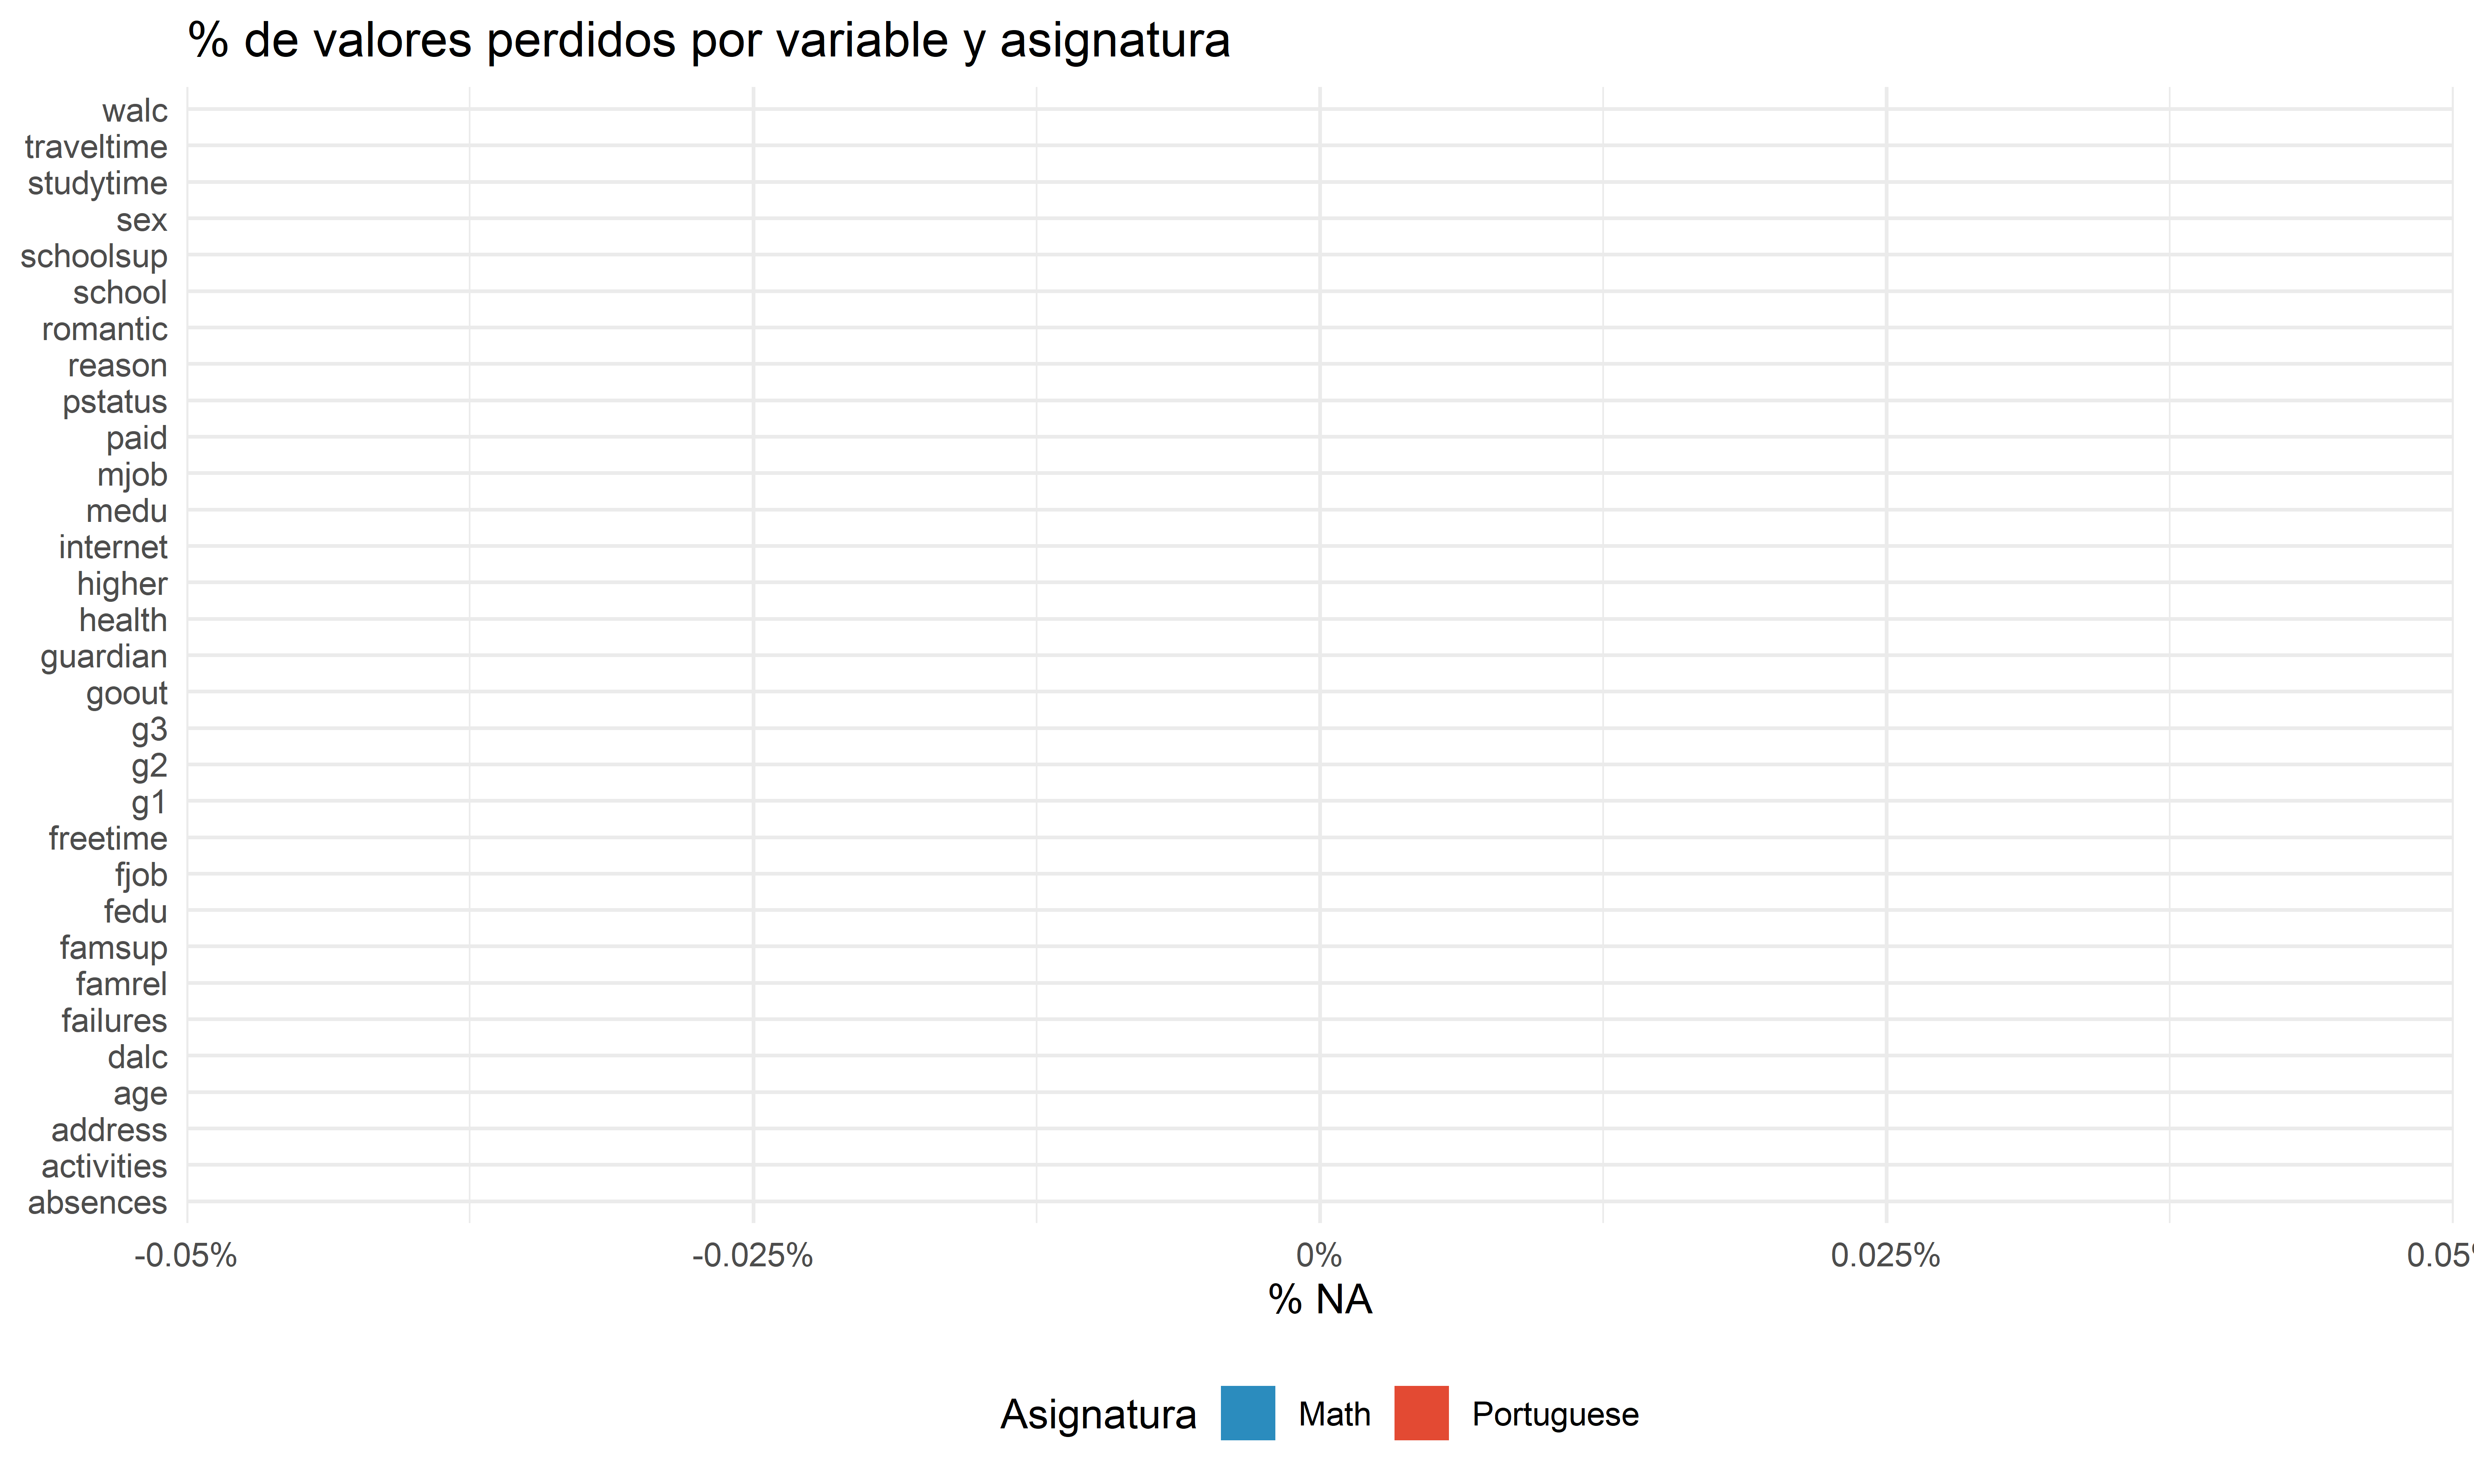
\includegraphics[keepaspectratio]{bookdown-demo_files/figure-latex/missing-visualization-1.pdf}}
\caption{\label{fig:missing-visualization}Análisis visual de valores perdidos por materia}
\end{figure}

\textbf{Conclusión sobre Missingness:}
Los datos están completos, sin valores perdidos, lo que indica una excelente calidad en la recolección de información. Esto elimina la necesidad de técnicas de imputación y permite proceder directamente con el análisis.

\begin{center}\rule{0.5\linewidth}{0.5pt}\end{center}

\section{4. Análisis Univariado: Rendimiento Académico (G3)}\label{anuxe1lisis-univariado-rendimiento-acaduxe9mico-g3}

\subsection{4.1 Estadísticas Descriptivas de G3}\label{estaduxedsticas-descriptivas-de-g3}

\begin{Shaded}
\begin{Highlighting}[]
\CommentTok{\# Estadísticas descriptivas por materia}
\NormalTok{g3\_stats }\OtherTok{\textless{}{-}}\NormalTok{ df\_all }\SpecialCharTok{\%\textgreater{}\%} 
  \FunctionTok{group\_by}\NormalTok{(subject) }\SpecialCharTok{\%\textgreater{}\%}
  \FunctionTok{summarise}\NormalTok{(}
    \AttributeTok{n =} \FunctionTok{n}\NormalTok{(),}
    \AttributeTok{media =} \FunctionTok{mean}\NormalTok{(g3),}
    \AttributeTok{desv\_std =} \FunctionTok{sd}\NormalTok{(g3),}
    \AttributeTok{mediana =} \FunctionTok{median}\NormalTok{(g3),}
    \AttributeTok{q1 =} \FunctionTok{quantile}\NormalTok{(g3, .}\DecValTok{25}\NormalTok{),}
    \AttributeTok{q3 =} \FunctionTok{quantile}\NormalTok{(g3, .}\DecValTok{75}\NormalTok{),}
    \AttributeTok{minimo =} \FunctionTok{min}\NormalTok{(g3),}
    \AttributeTok{maximo =} \FunctionTok{max}\NormalTok{(g3),}
    \AttributeTok{.groups =} \StringTok{"drop"}
\NormalTok{  )}

\FunctionTok{kable}\NormalTok{(g3\_stats, }
      \AttributeTok{caption =} \StringTok{"Estadísticas descriptivas de G3 por materia"}\NormalTok{,}
      \AttributeTok{digits =} \DecValTok{2}\NormalTok{,}
      \AttributeTok{col.names =} \FunctionTok{c}\NormalTok{(}\StringTok{"Materia"}\NormalTok{, }\StringTok{"N"}\NormalTok{, }\StringTok{"Media"}\NormalTok{, }\StringTok{"Desv.Std"}\NormalTok{, }\StringTok{"Mediana"}\NormalTok{, }\StringTok{"Q1"}\NormalTok{, }\StringTok{"Q3"}\NormalTok{, }\StringTok{"Mín"}\NormalTok{, }\StringTok{"Máx"}\NormalTok{))}
\end{Highlighting}
\end{Shaded}

\begin{table}

\caption{\label{tab:g3-descriptives}Estadísticas descriptivas de G3 por materia}
\centering
\begin{tabular}[t]{l|r|r|r|r|r|r|r|r}
\hline
Materia & N & Media & Desv.Std & Mediana & Q1 & Q3 & Mín & Máx\\
\hline
Math & 395 & 10.42 & 4.58 & 11 & 8 & 14 & 0 & 20\\
\hline
Portuguese & 649 & 11.91 & 3.23 & 12 & 10 & 14 & 0 & 19\\
\hline
\end{tabular}
\end{table}

\subsection{4.2 Distribución de Calificaciones}\label{distribuciuxf3n-de-calificaciones}

\begin{Shaded}
\begin{Highlighting}[]
\CommentTok{\# Comparación directa con boxplot}
\FunctionTok{boxplot}\NormalTok{(mat}\SpecialCharTok{$}\NormalTok{g3, por}\SpecialCharTok{$}\NormalTok{g3,}
        \AttributeTok{names =} \FunctionTok{c}\NormalTok{(}\StringTok{"Math"}\NormalTok{, }\StringTok{"Portuguese"}\NormalTok{),}
        \AttributeTok{main =} \StringTok{"G3 — Comparación entre asignaturas"}\NormalTok{,}
        \AttributeTok{col =} \FunctionTok{c}\NormalTok{(pal[}\StringTok{"Math"}\NormalTok{], pal[}\StringTok{"Portuguese"}\NormalTok{]),}
        \AttributeTok{ylab =} \StringTok{"Calificación Final (G3)"}\NormalTok{)}
\end{Highlighting}
\end{Shaded}

\begin{figure}
\centering
\pandocbounded{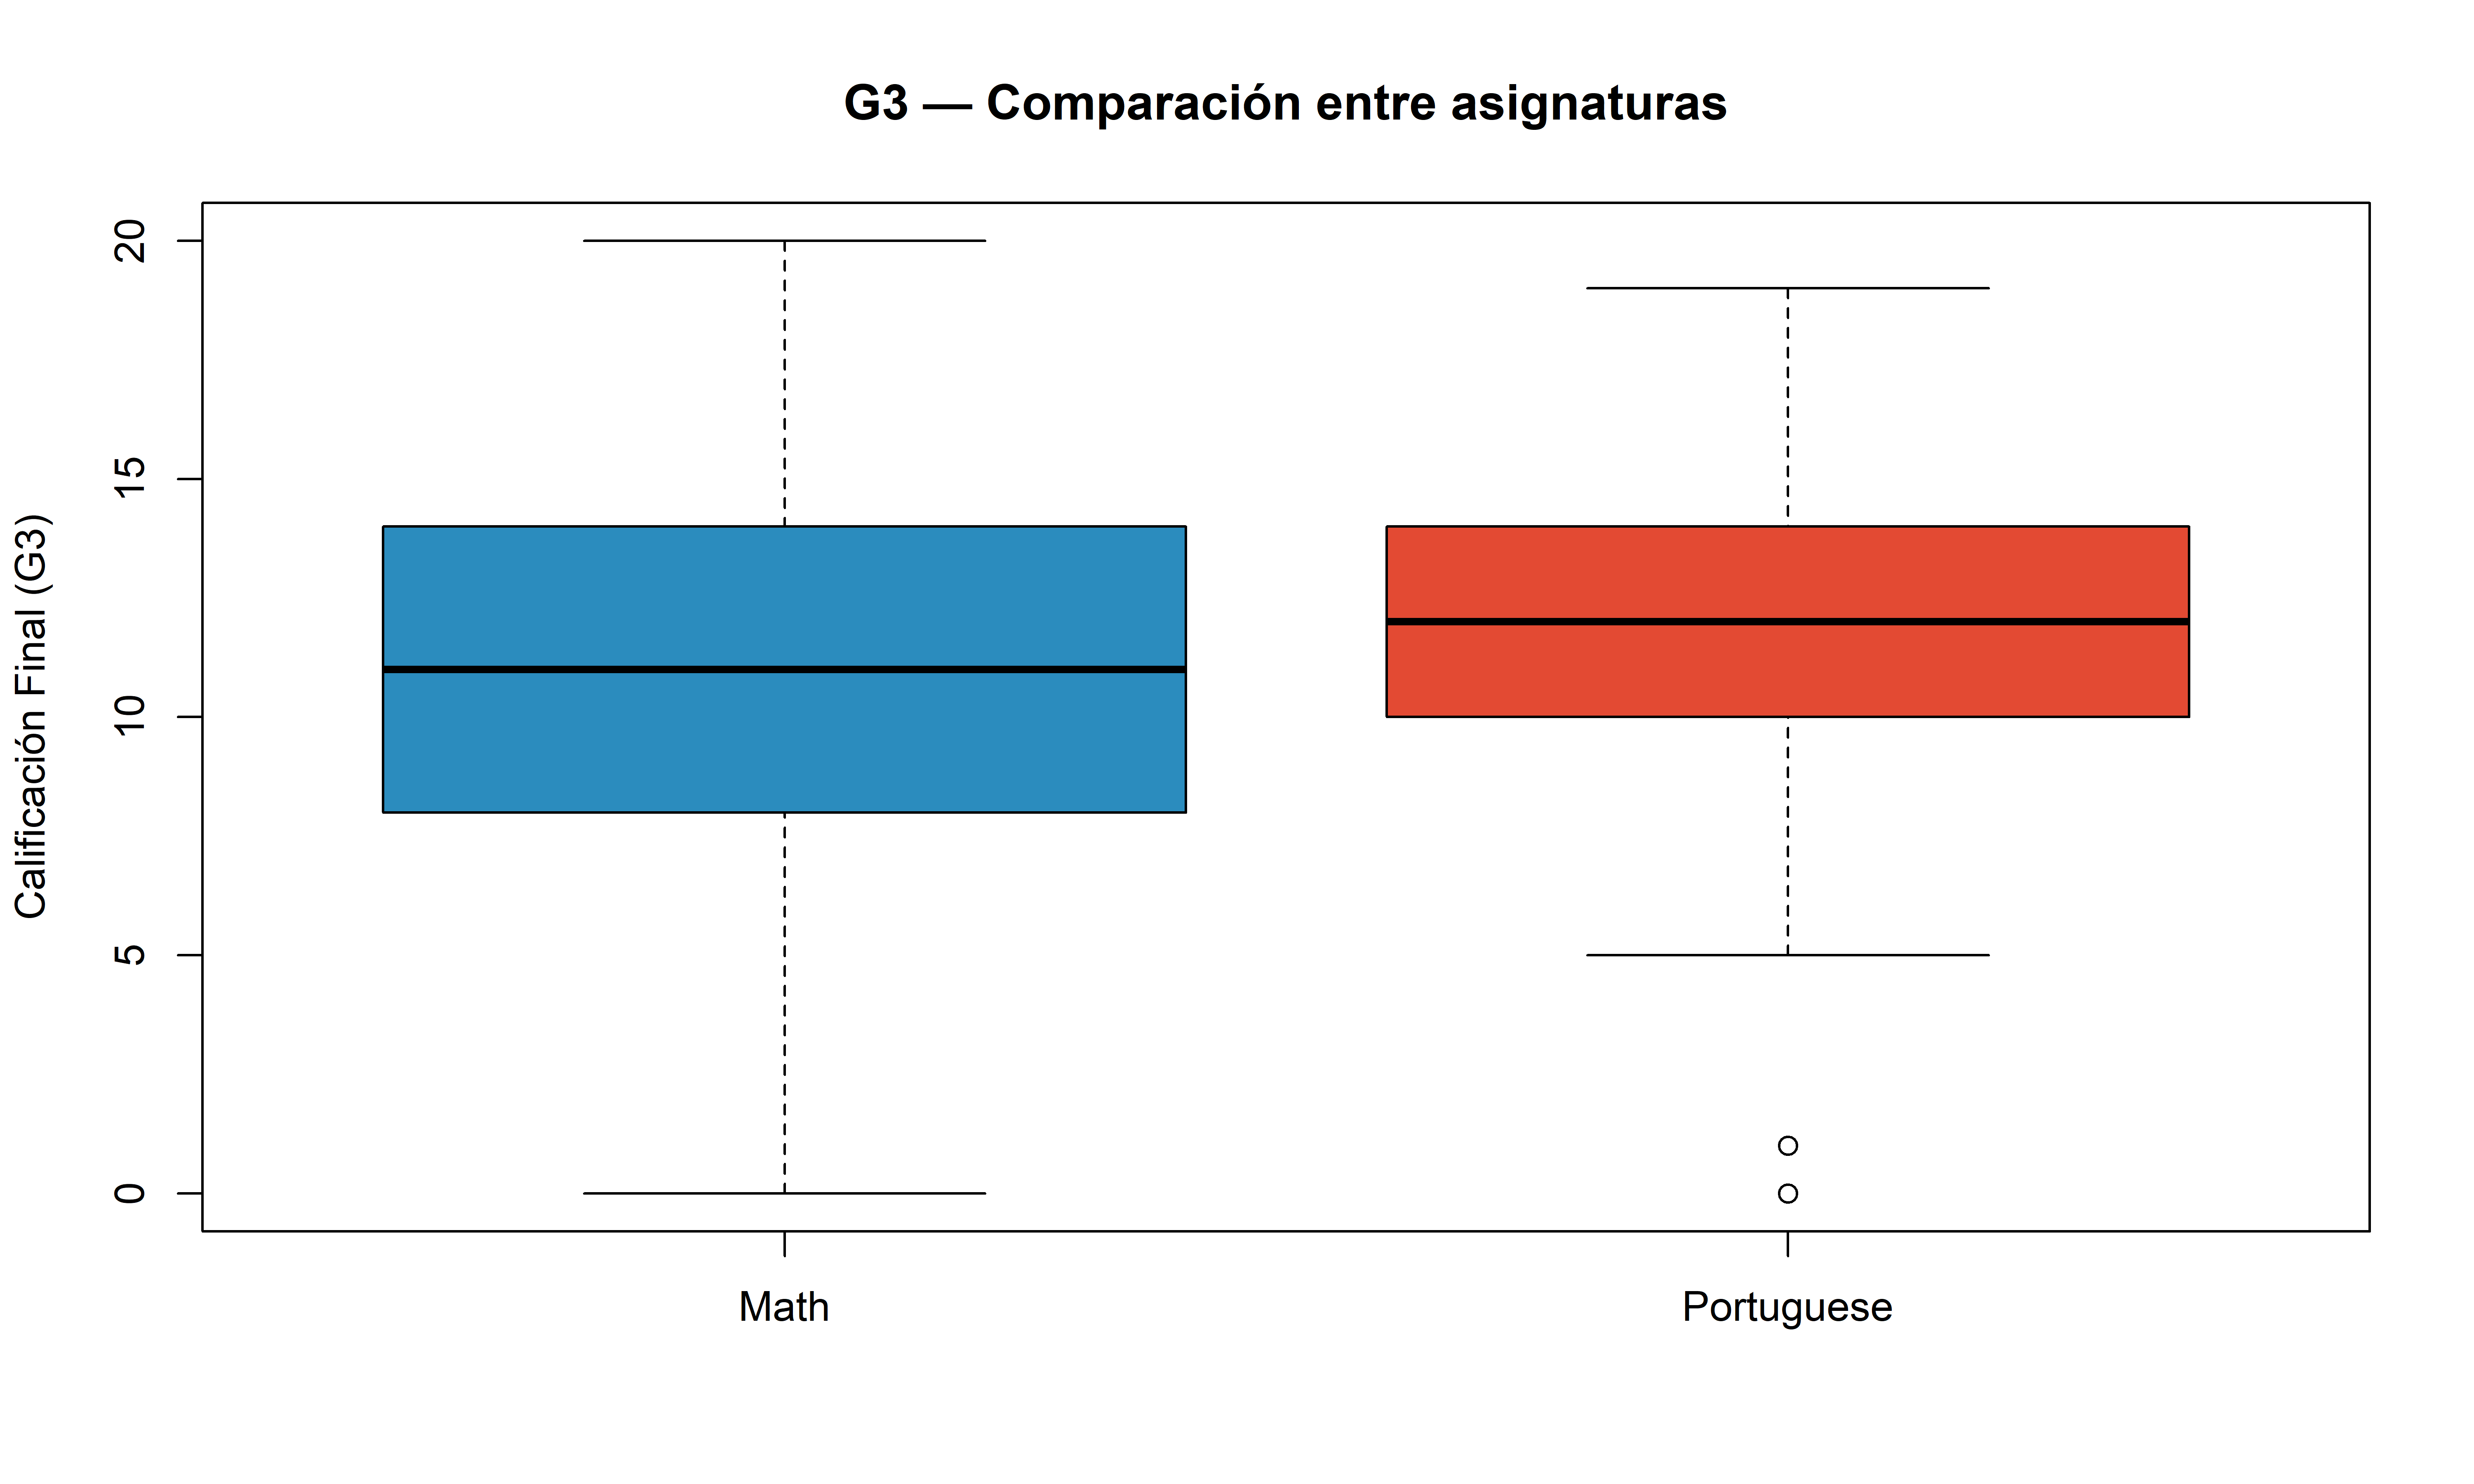
\includegraphics[keepaspectratio]{bookdown-demo_files/figure-latex/g3-distribution-1.pdf}}
\caption{\label{fig:g3-distribution-1}Distribución de calificaciones finales (G3) por materia}
\end{figure}

\begin{Shaded}
\begin{Highlighting}[]
\CommentTok{\# Histograma comparativo}
\NormalTok{p1 }\OtherTok{\textless{}{-}} \FunctionTok{ggplot}\NormalTok{(df\_all, }\FunctionTok{aes}\NormalTok{(g3, }\AttributeTok{fill =}\NormalTok{ subject)) }\SpecialCharTok{+}
  \FunctionTok{geom\_histogram}\NormalTok{(}\AttributeTok{bins =} \DecValTok{30}\NormalTok{, }\AttributeTok{position =} \StringTok{"identity"}\NormalTok{, }\AttributeTok{alpha =}\NormalTok{ .}\DecValTok{55}\NormalTok{) }\SpecialCharTok{+}
  \FunctionTok{facet\_wrap}\NormalTok{(}\SpecialCharTok{\textasciitilde{}}\NormalTok{subject, }\AttributeTok{ncol =} \DecValTok{1}\NormalTok{) }\SpecialCharTok{+}
  \FunctionTok{scale\_fill\_manual}\NormalTok{(}\AttributeTok{values =}\NormalTok{ pal) }\SpecialCharTok{+}
  \FunctionTok{labs}\NormalTok{(}\AttributeTok{title =} \StringTok{"Distribución de G3 por asignatura"}\NormalTok{, }\AttributeTok{x =} \StringTok{"G3"}\NormalTok{, }\AttributeTok{y =} \StringTok{"Frecuencia"}\NormalTok{) }\SpecialCharTok{+}
  \FunctionTok{theme}\NormalTok{(}\AttributeTok{legend.position =} \StringTok{"none"}\NormalTok{)}

\CommentTok{\# Gráfico de densidad}
\NormalTok{p2 }\OtherTok{\textless{}{-}} \FunctionTok{ggplot}\NormalTok{(df\_all, }\FunctionTok{aes}\NormalTok{(g3, }\AttributeTok{color =}\NormalTok{ subject)) }\SpecialCharTok{+}
  \FunctionTok{geom\_density}\NormalTok{(}\AttributeTok{linewidth =} \FloatTok{1.2}\NormalTok{) }\SpecialCharTok{+}
  \FunctionTok{scale\_color\_manual}\NormalTok{(}\AttributeTok{values =}\NormalTok{ pal) }\SpecialCharTok{+}
  \FunctionTok{labs}\NormalTok{(}\AttributeTok{title =} \StringTok{"Densidad de G3 por asignatura"}\NormalTok{, }\AttributeTok{x =} \StringTok{"G3"}\NormalTok{, }\AttributeTok{y =} \StringTok{"Densidad"}\NormalTok{) }\SpecialCharTok{+}
  \FunctionTok{theme}\NormalTok{(}\AttributeTok{legend.position =} \StringTok{"bottom"}\NormalTok{)}

\FunctionTok{print}\NormalTok{(p1)}
\end{Highlighting}
\end{Shaded}

\begin{figure}
\centering
\pandocbounded{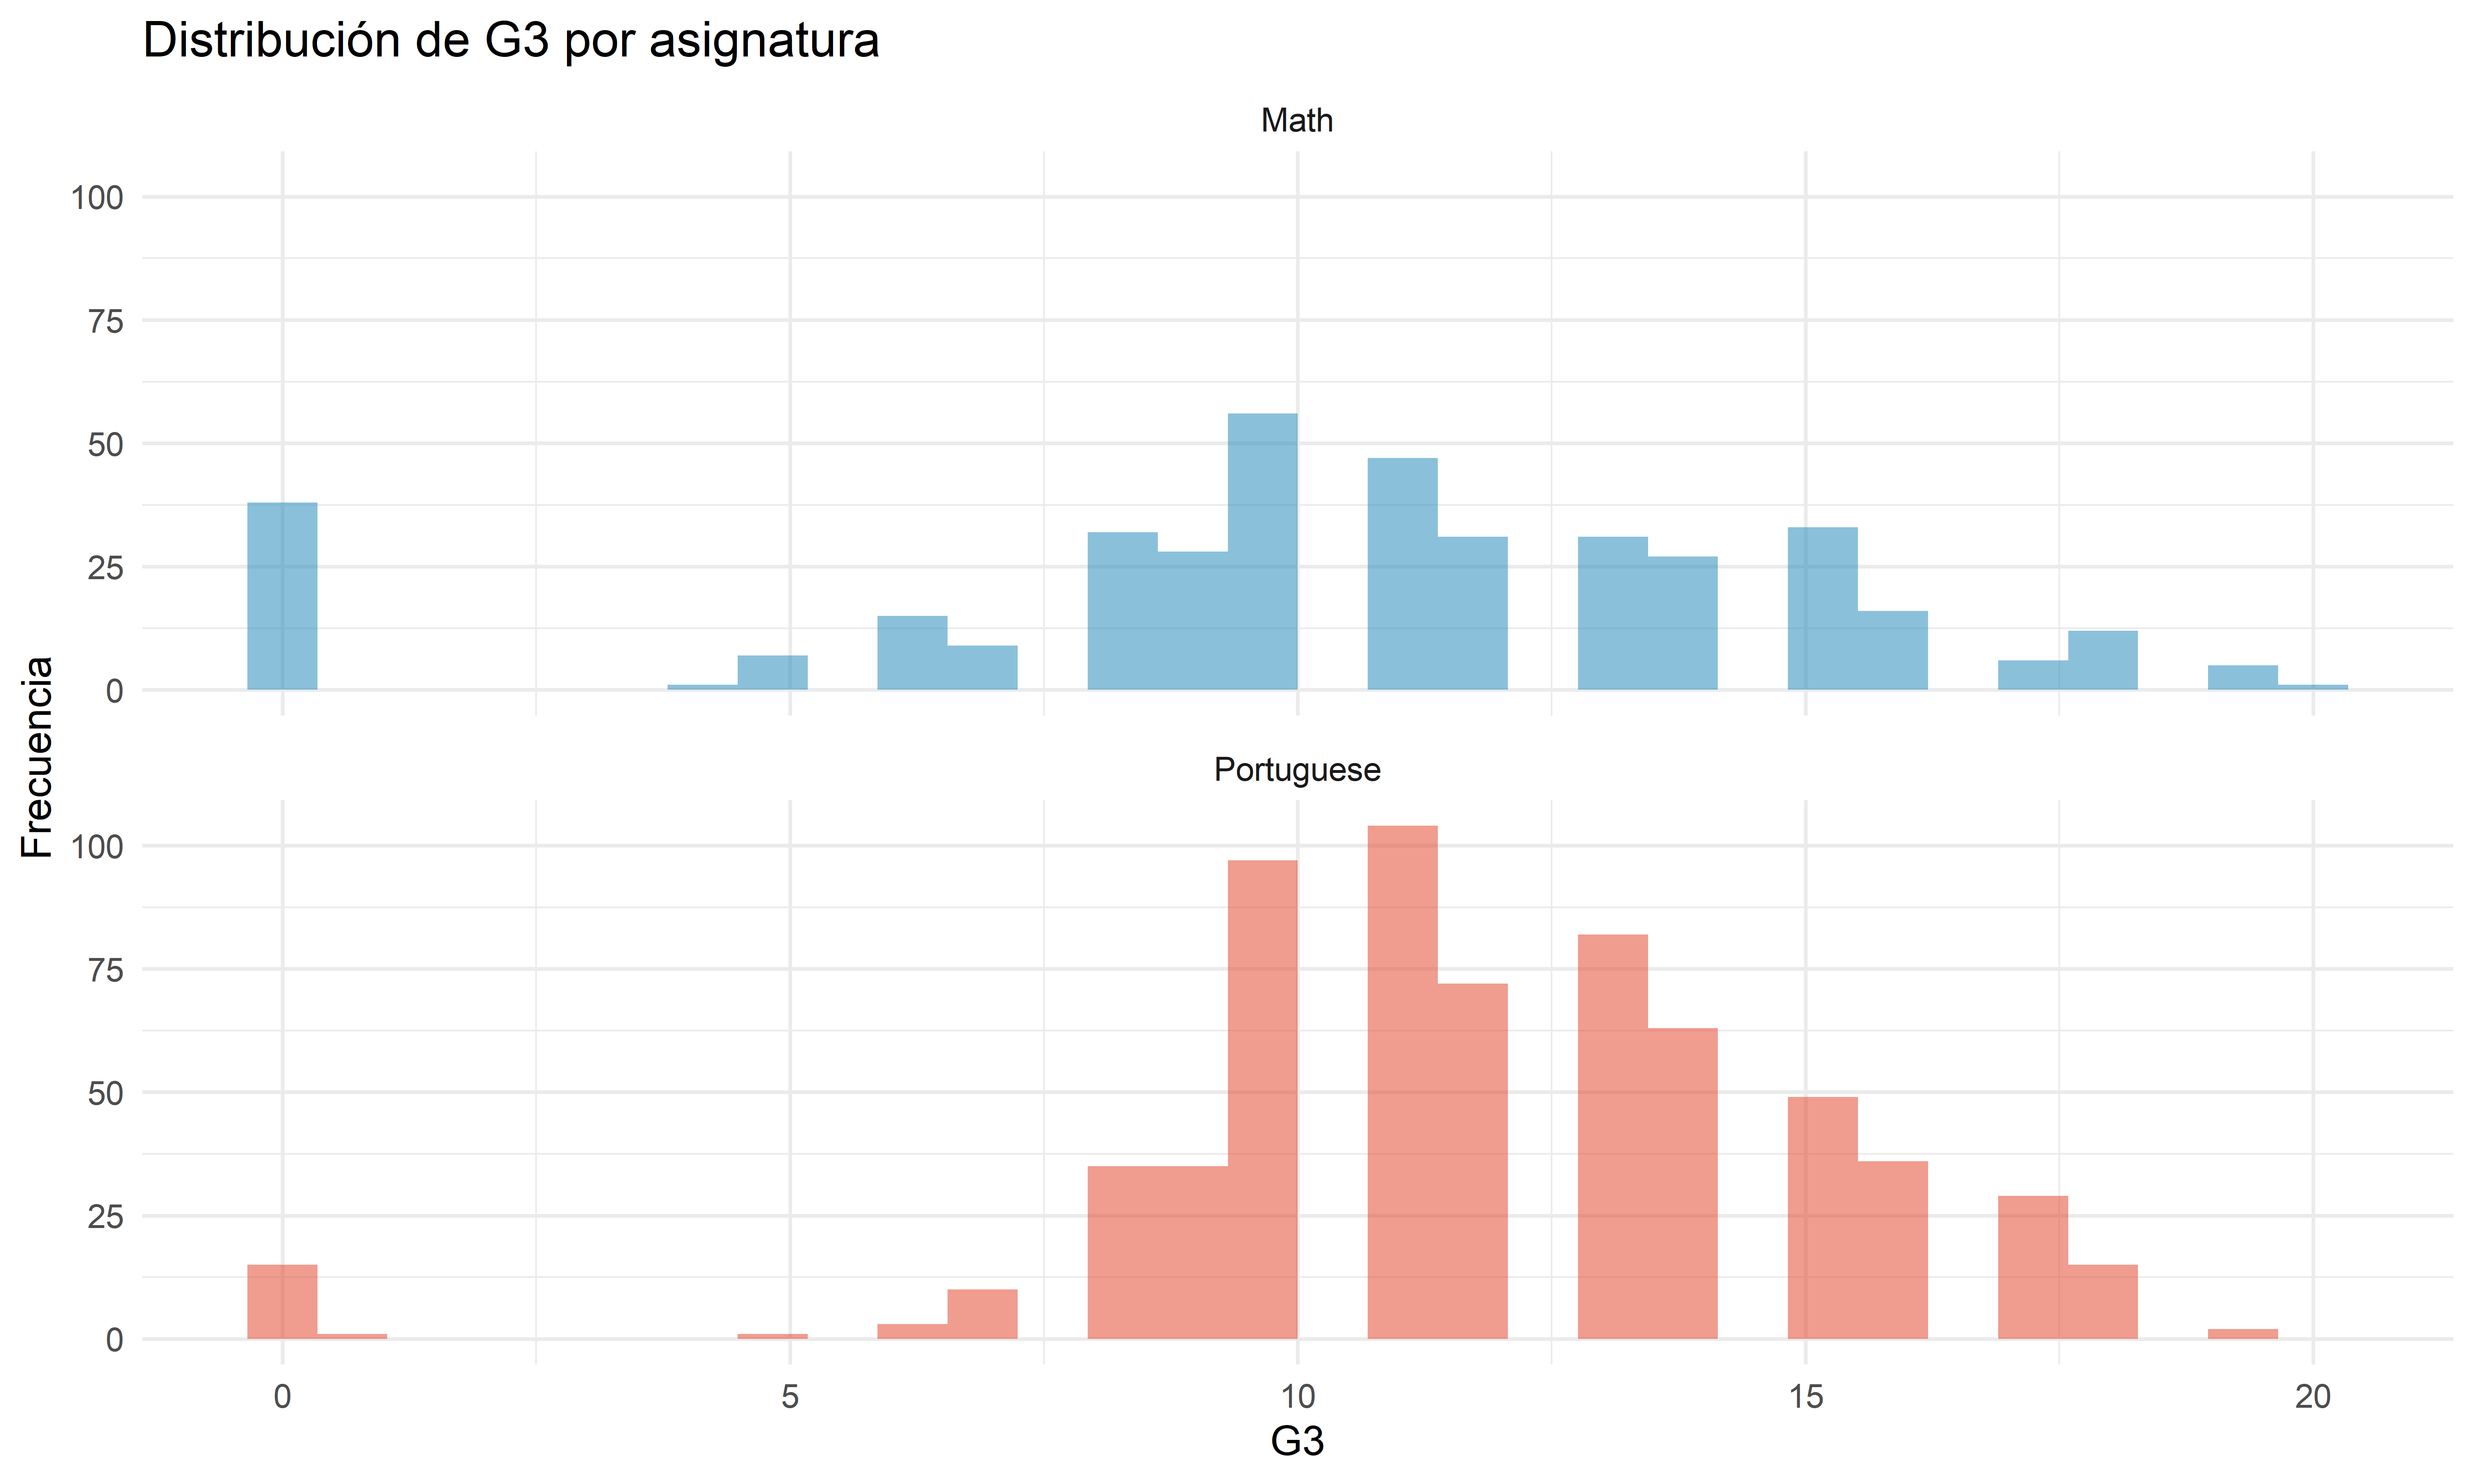
\includegraphics[keepaspectratio]{bookdown-demo_files/figure-latex/g3-distribution-2.pdf}}
\caption{\label{fig:g3-distribution-2}Distribución de calificaciones finales (G3) por materia}
\end{figure}

\begin{Shaded}
\begin{Highlighting}[]
\FunctionTok{print}\NormalTok{(p2)}
\end{Highlighting}
\end{Shaded}

\begin{figure}
\centering
\pandocbounded{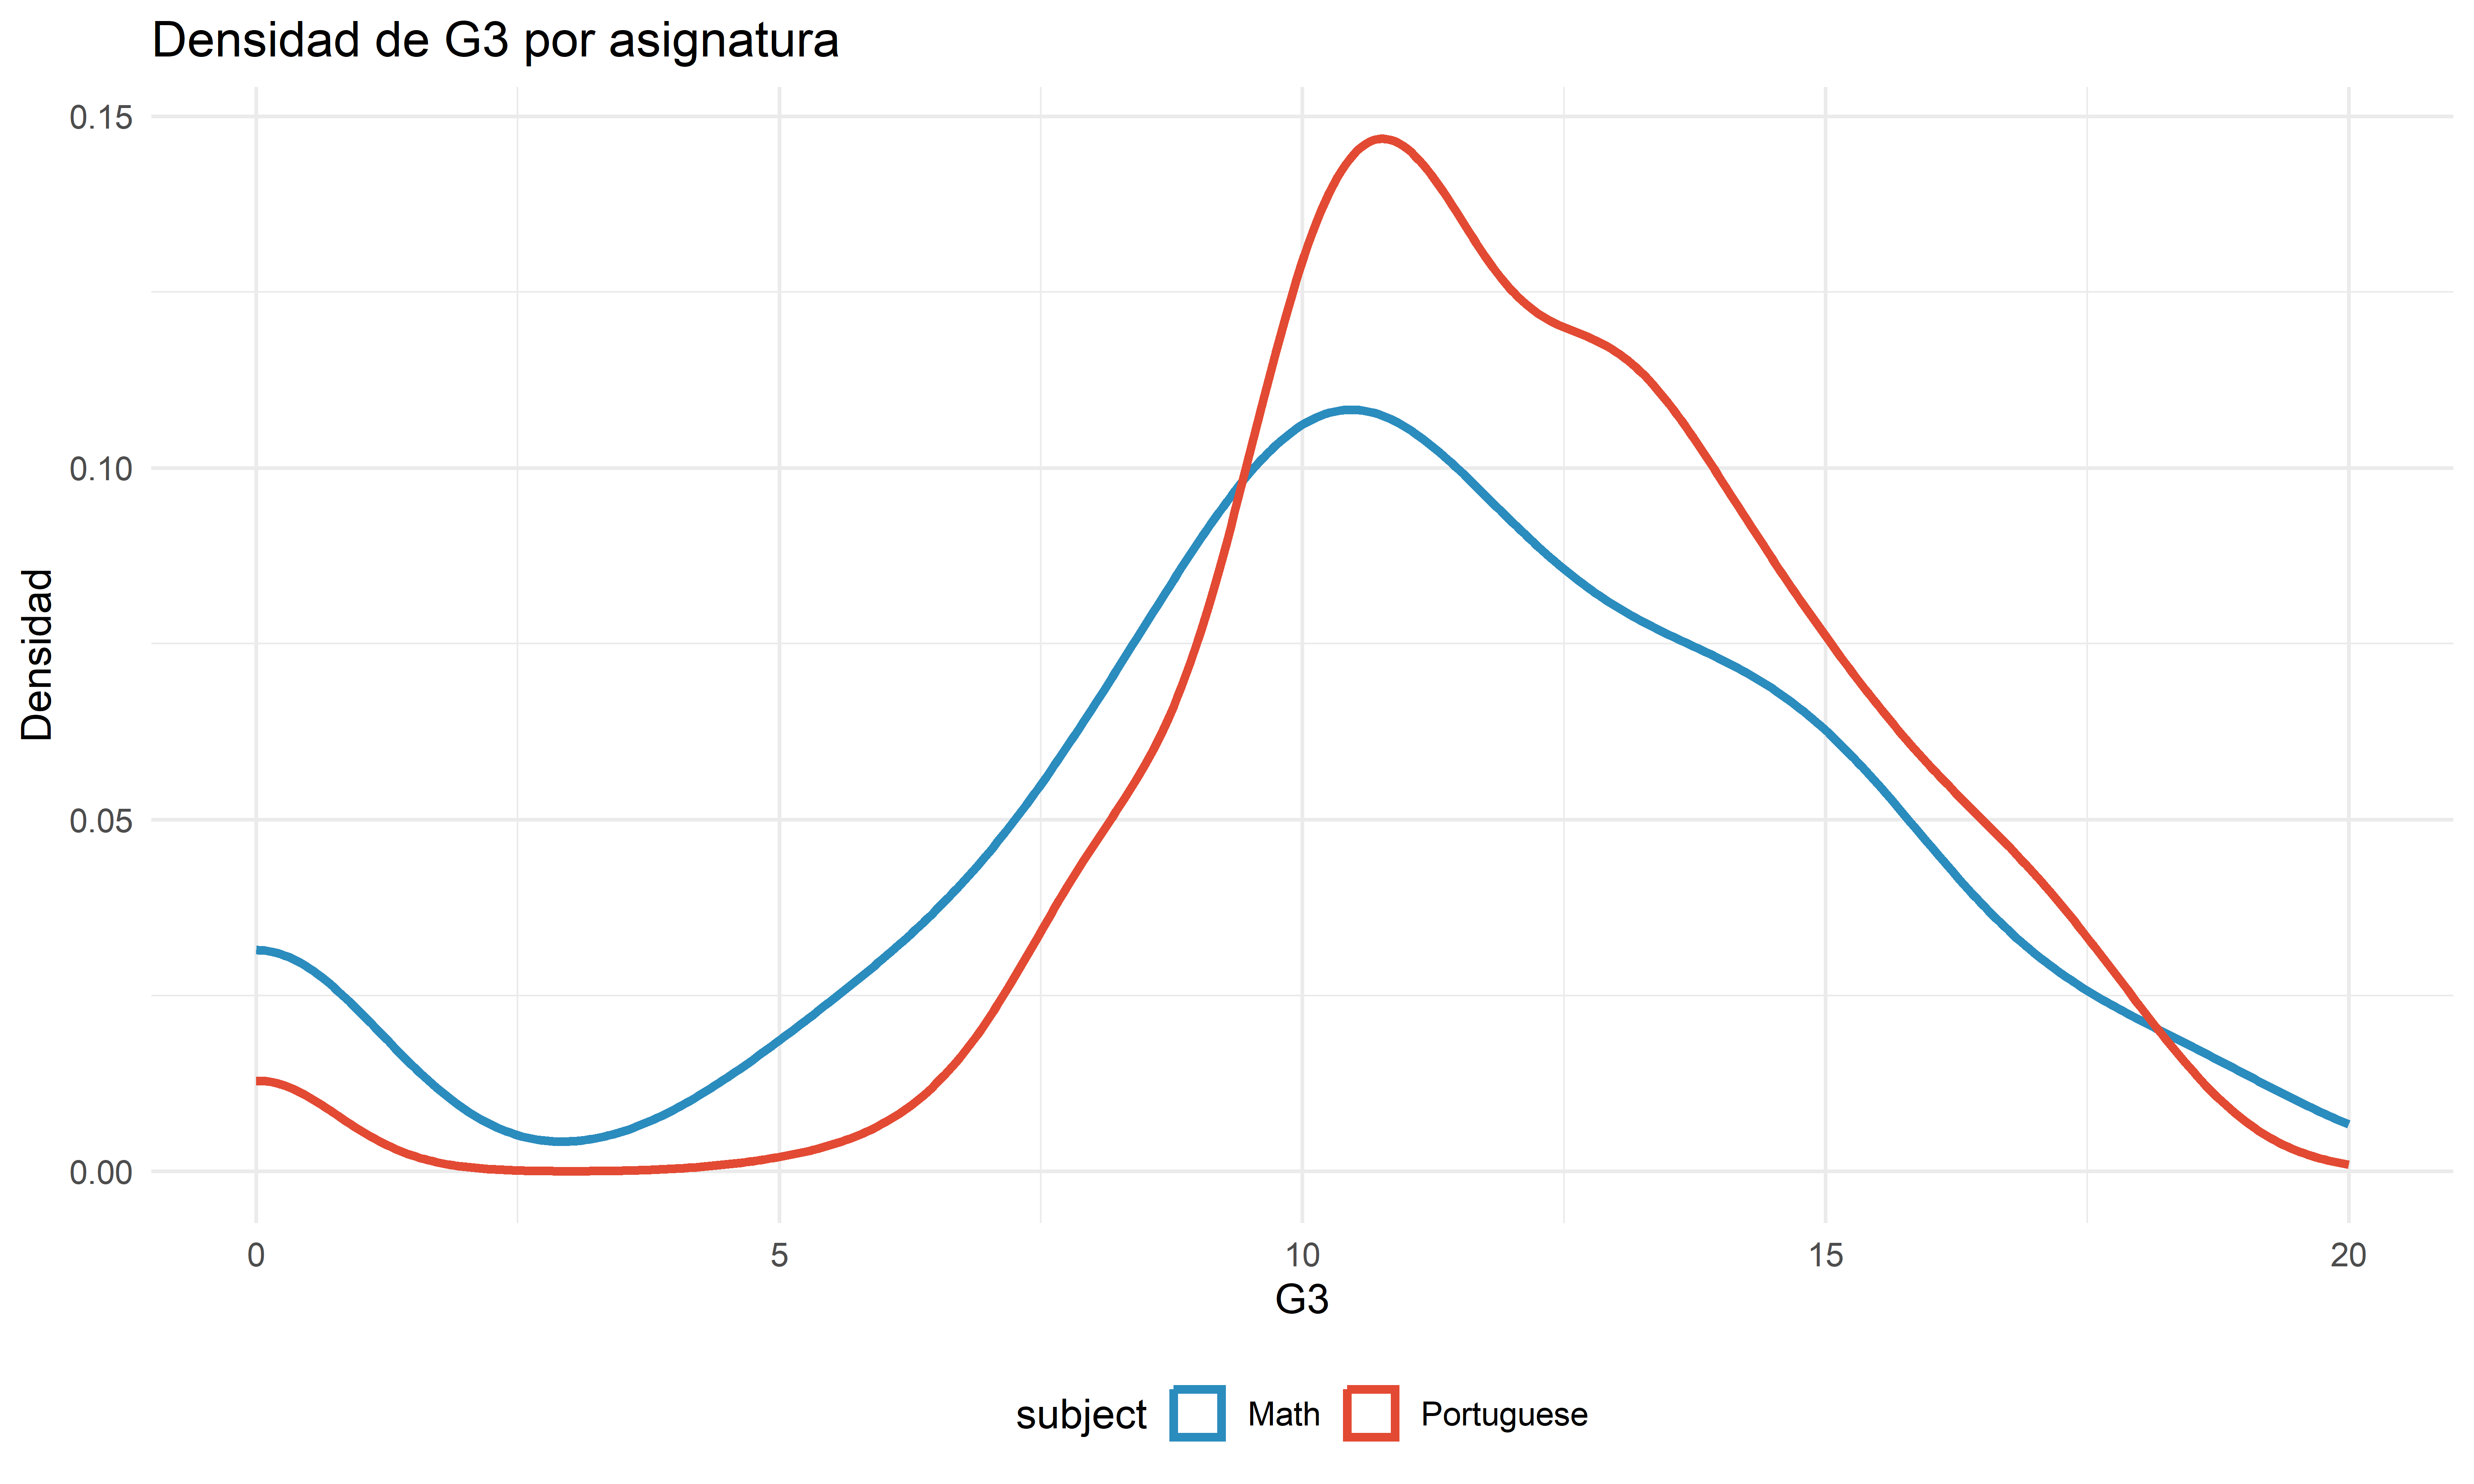
\includegraphics[keepaspectratio]{bookdown-demo_files/figure-latex/g3-distribution-3.pdf}}
\caption{\label{fig:g3-distribution-3}Distribución de calificaciones finales (G3) por materia}
\end{figure}

\textbf{Análisis del Rendimiento por Materia:}

\begin{itemize}
\tightlist
\item
  \textbf{Matemáticas:} Media de 10.42 con desviación estándar de 4.58
\item
  \textbf{Portugués:} Media de 11.91 con desviación estándar de 3.23
\end{itemize}

\textbf{Deducción clave:} Los estudiantes obtienen calificaciones significativamente más altas en Portugués que en Matemáticas, sugiriendo que Matemáticas presenta mayor dificultad académica o que los estudiantes tienen mejor dominio de su lengua materna.

\begin{center}\rule{0.5\linewidth}{0.5pt}\end{center}

\section{5. Análisis Multivariado: Panel Exploratorio}\label{anuxe1lisis-multivariado-panel-exploratorio}

\subsection{5.1 Matriz de Correlaciones y Relaciones}\label{matriz-de-correlaciones-y-relaciones}

\begin{Shaded}
\begin{Highlighting}[]
\CommentTok{\# Variables clave para análisis}
\NormalTok{nums\_key }\OtherTok{\textless{}{-}} \FunctionTok{intersect}\NormalTok{(}\FunctionTok{c}\NormalTok{(}\StringTok{"g3"}\NormalTok{,}\StringTok{"g2"}\NormalTok{,}\StringTok{"g1"}\NormalTok{,}\StringTok{"studytime"}\NormalTok{,}\StringTok{"failures"}\NormalTok{,}\StringTok{"absences"}\NormalTok{,}\StringTok{"age"}\NormalTok{), }\FunctionTok{names}\NormalTok{(df\_all))}
\NormalTok{vars\_panel }\OtherTok{\textless{}{-}} \FunctionTok{unique}\NormalTok{(}\FunctionTok{c}\NormalTok{(nums\_key, }\FunctionTok{intersect}\NormalTok{(}\StringTok{"sex"}\NormalTok{, }\FunctionTok{names}\NormalTok{(df\_all))))}
\NormalTok{df\_small }\OtherTok{\textless{}{-}}\NormalTok{ df\_all[, }\FunctionTok{unique}\NormalTok{(}\FunctionTok{c}\NormalTok{(vars\_panel, }\StringTok{"subject"}\NormalTok{))]}

\CommentTok{\# Panel multivariado con GGally}
\NormalTok{p\_mix }\OtherTok{\textless{}{-}} \FunctionTok{ggpairs}\NormalTok{(}
\NormalTok{  df\_small,}
  \AttributeTok{mapping =}\NormalTok{ ggplot2}\SpecialCharTok{::}\FunctionTok{aes}\NormalTok{(}\AttributeTok{color =}\NormalTok{ subject, }\AttributeTok{alpha =} \FloatTok{0.55}\NormalTok{),}
  \AttributeTok{upper =} \FunctionTok{list}\NormalTok{(}
    \AttributeTok{continuous =} \FunctionTok{wrap}\NormalTok{(}\StringTok{"cor"}\NormalTok{, }\AttributeTok{size =} \DecValTok{3}\NormalTok{),    }\CommentTok{\# Correlaciones en triángulo superior}
    \AttributeTok{combo      =} \StringTok{"box\_no\_facet"}\NormalTok{,           }\CommentTok{\# Boxplots para cat\textasciitilde{}num}
    \AttributeTok{discrete   =} \StringTok{"blank"}                   \CommentTok{\# Espacio en blanco para cat\textasciitilde{}cat}
\NormalTok{  ),}
  \AttributeTok{lower =} \FunctionTok{list}\NormalTok{(}
    \AttributeTok{continuous =} \FunctionTok{wrap}\NormalTok{(}\StringTok{"points"}\NormalTok{, }\AttributeTok{alpha =}\NormalTok{ .}\DecValTok{35}\NormalTok{, }\AttributeTok{size =}\NormalTok{ .}\DecValTok{6}\NormalTok{),  }\CommentTok{\# Scatter plots}
    \AttributeTok{combo      =} \StringTok{"facethist"}\NormalTok{,              }\CommentTok{\# Histogramas por facetas}
    \AttributeTok{discrete   =} \StringTok{"count"}                   \CommentTok{\# Conteos para cat\textasciitilde{}cat}
\NormalTok{  ),}
  \AttributeTok{diag  =} \FunctionTok{list}\NormalTok{(}\AttributeTok{continuous =} \StringTok{"densityDiag"}\NormalTok{), }\CommentTok{\# Densidades en diagonal}
  \AttributeTok{title =} \StringTok{"Exploración compacta — Variables clave (coloreado por asignatura)"}
\NormalTok{) }\SpecialCharTok{+} \FunctionTok{theme}\NormalTok{(}\AttributeTok{legend.position =} \StringTok{"bottom"}\NormalTok{)}

\FunctionTok{print}\NormalTok{(p\_mix)}
\end{Highlighting}
\end{Shaded}

\begin{figure}
\centering
\pandocbounded{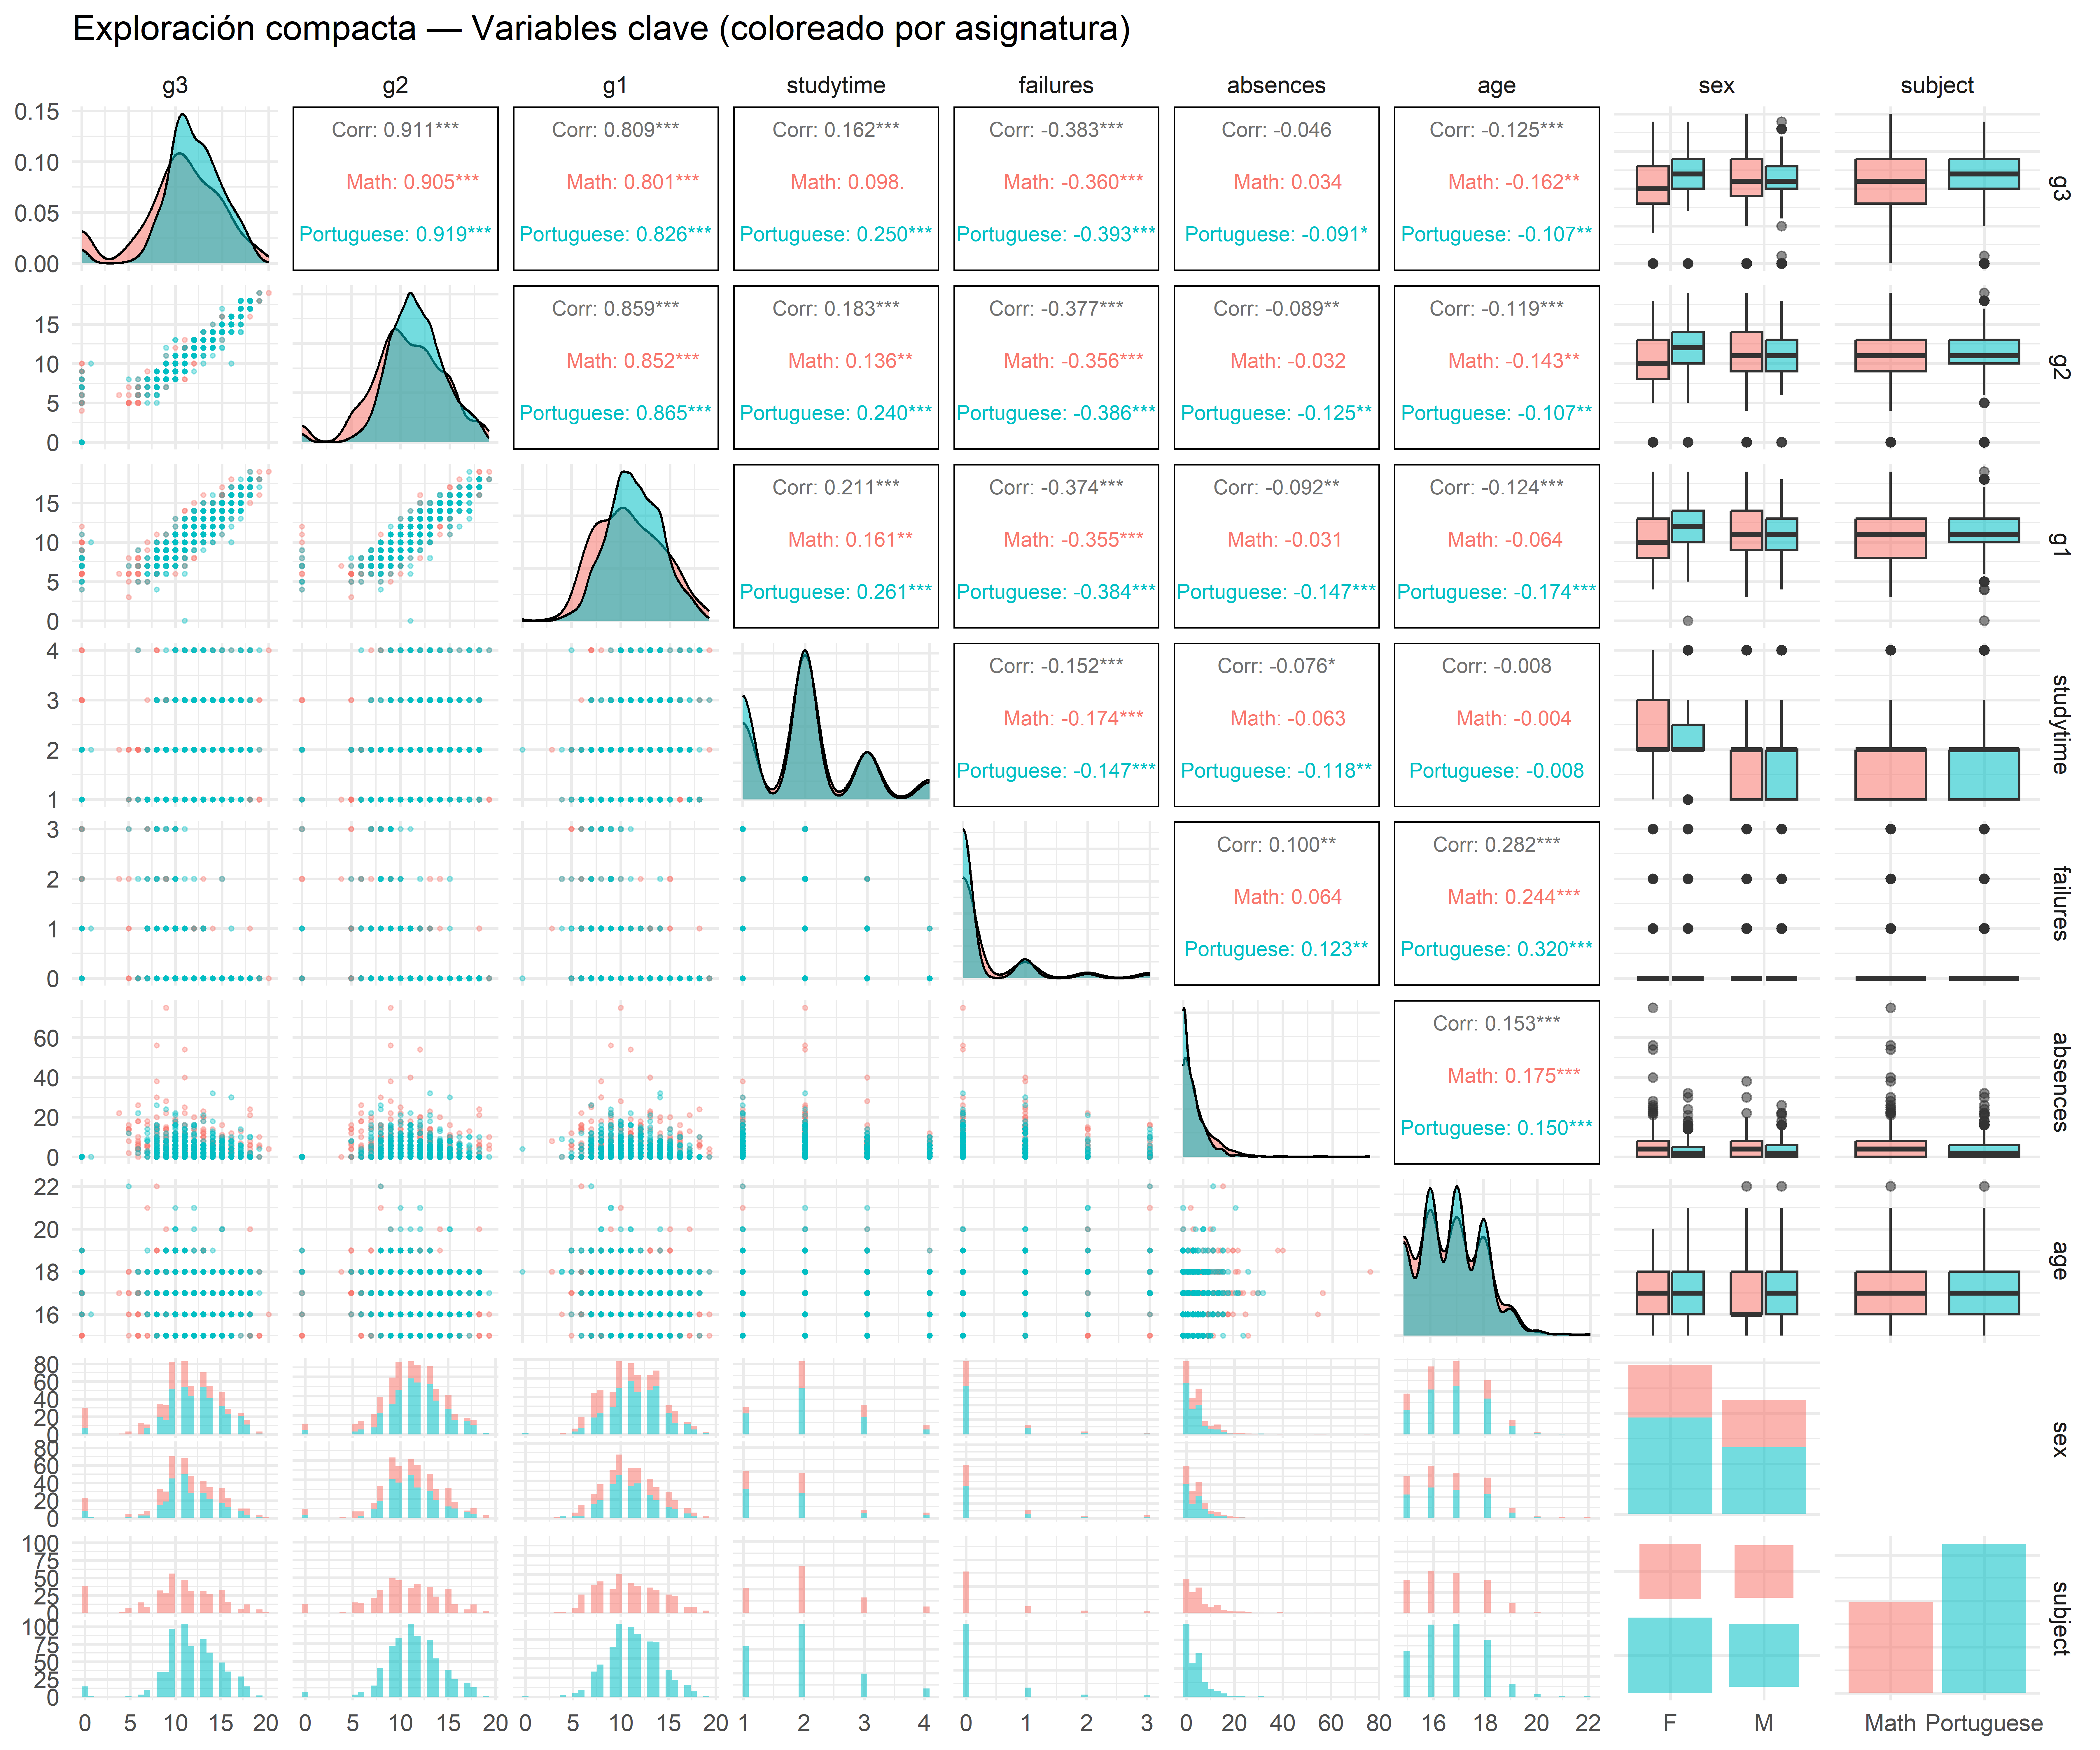
\includegraphics[keepaspectratio]{bookdown-demo_files/figure-latex/correlation-panel-1.pdf}}
\caption{\label{fig:correlation-panel}Panel exploratorio multivariado - Variables clave coloreadas por materia}
\end{figure}

\textbf{Interpretación del Panel Multivariado:}

\begin{enumerate}
\def\labelenumi{\arabic{enumi}.}
\item
  \textbf{Correlaciones G1-G2-G3:} Se observan correlaciones muy altas (\textgreater0.8) entre las calificaciones de los tres períodos, indicando consistencia en el rendimiento estudiantil a lo largo del año académico.
\item
  \textbf{Impacto de Failures:} Las correlaciones negativas con las calificaciones finales sugieren que el historial de reprobaciones es un predictor fuerte del rendimiento actual.
\item
  \textbf{Diferencias por Materia:} Los patrones de dispersión muestran variaciones sistemáticas entre Matemáticas y Portugués en múltiples variables.
\end{enumerate}

\begin{center}\rule{0.5\linewidth}{0.5pt}\end{center}

\section{6. Análisis Bivariado Detallado}\label{anuxe1lisis-bivariado-detallado}

\subsection{6.1 Variables Numéricas vs Rendimiento}\label{variables-numuxe9ricas-vs-rendimiento}

\begin{Shaded}
\begin{Highlighting}[]
\CommentTok{\# Variables numéricas clave excluyendo G3}
\NormalTok{numeric\_predictors }\OtherTok{\textless{}{-}} \FunctionTok{setdiff}\NormalTok{(numeric\_vars, }\StringTok{"g3"}\NormalTok{)}

\CommentTok{\# Análisis de correlaciones}
\NormalTok{correlations }\OtherTok{\textless{}{-}}\NormalTok{ df\_all }\SpecialCharTok{\%\textgreater{}\%}
  \FunctionTok{select}\NormalTok{(subject, }\FunctionTok{all\_of}\NormalTok{(numeric\_predictors), g3) }\SpecialCharTok{\%\textgreater{}\%}
  \FunctionTok{group\_by}\NormalTok{(subject) }\SpecialCharTok{\%\textgreater{}\%}
  \FunctionTok{summarise}\NormalTok{(}
    \FunctionTok{across}\NormalTok{(}\FunctionTok{all\_of}\NormalTok{(numeric\_predictors), }\SpecialCharTok{\textasciitilde{}}\FunctionTok{cor}\NormalTok{(., g3, }\AttributeTok{use =} \StringTok{"complete.obs"}\NormalTok{)),}
    \AttributeTok{.groups =} \StringTok{"drop"}
\NormalTok{  )}

\CommentTok{\# Tabla de correlaciones}
\NormalTok{cor\_table }\OtherTok{\textless{}{-}}\NormalTok{ correlations }\SpecialCharTok{\%\textgreater{}\%}
  \FunctionTok{pivot\_longer}\NormalTok{(}\SpecialCharTok{{-}}\NormalTok{subject, }\AttributeTok{names\_to =} \StringTok{"variable"}\NormalTok{, }\AttributeTok{values\_to =} \StringTok{"correlation"}\NormalTok{) }\SpecialCharTok{\%\textgreater{}\%}
  \FunctionTok{pivot\_wider}\NormalTok{(}\AttributeTok{names\_from =}\NormalTok{ subject, }\AttributeTok{values\_from =}\NormalTok{ correlation) }\SpecialCharTok{\%\textgreater{}\%}
  \FunctionTok{arrange}\NormalTok{(}\FunctionTok{desc}\NormalTok{(}\FunctionTok{abs}\NormalTok{(Math }\SpecialCharTok{+}\NormalTok{ Portuguese)))}

\FunctionTok{kable}\NormalTok{(cor\_table, }
      \AttributeTok{caption =} \StringTok{"Correlaciones entre variables numéricas y G3 por materia"}\NormalTok{,}
      \AttributeTok{digits =} \DecValTok{3}\NormalTok{,}
      \AttributeTok{col.names =} \FunctionTok{c}\NormalTok{(}\StringTok{"Variable"}\NormalTok{, }\StringTok{"Matemáticas"}\NormalTok{, }\StringTok{"Portugués"}\NormalTok{))}
\end{Highlighting}
\end{Shaded}

\begin{table}

\caption{\label{tab:numeric-bivariate}Correlaciones entre variables numéricas y G3 por materia}
\centering
\begin{tabular}[t]{l|r|r}
\hline
Variable & Matemáticas & Portugués\\
\hline
g2 & 0.905 & 0.919\\
\hline
g1 & 0.801 & 0.826\\
\hline
failures & -0.360 & -0.393\\
\hline
medu & 0.217 & 0.240\\
\hline
fedu & 0.152 & 0.212\\
\hline
studytime & 0.098 & 0.250\\
\hline
age & -0.162 & -0.107\\
\hline
dalc & -0.055 & -0.205\\
\hline
traveltime & -0.117 & -0.127\\
\hline
walc & -0.052 & -0.177\\
\hline
goout & -0.133 & -0.088\\
\hline
health & -0.061 & -0.099\\
\hline
famrel & 0.051 & 0.063\\
\hline
freetime & 0.011 & -0.123\\
\hline
absences & 0.034 & -0.091\\
\hline
\end{tabular}
\end{table}

\begin{Shaded}
\begin{Highlighting}[]
\CommentTok{\# Gráficos de dispersión para variables más correlacionadas}
\NormalTok{top\_vars }\OtherTok{\textless{}{-}}\NormalTok{ cor\_table}\SpecialCharTok{$}\NormalTok{variable[}\DecValTok{1}\SpecialCharTok{:}\DecValTok{6}\NormalTok{]  }\CommentTok{\# Top 6 variables más correlacionadas}

\NormalTok{plots\_list }\OtherTok{\textless{}{-}} \FunctionTok{map}\NormalTok{(top\_vars, }\SpecialCharTok{\textasciitilde{}}\NormalTok{\{}
  \FunctionTok{ggplot}\NormalTok{(df\_all, }\FunctionTok{aes}\NormalTok{(.data[[.x]], g3, }\AttributeTok{color =}\NormalTok{ subject)) }\SpecialCharTok{+}
    \FunctionTok{geom\_point}\NormalTok{(}\AttributeTok{alpha =}\NormalTok{ .}\DecValTok{4}\NormalTok{, }\AttributeTok{size =} \DecValTok{1}\NormalTok{) }\SpecialCharTok{+}
    \FunctionTok{geom\_smooth}\NormalTok{(}\AttributeTok{method =} \StringTok{"lm"}\NormalTok{, }\AttributeTok{se =} \ConstantTok{FALSE}\NormalTok{, }\AttributeTok{linewidth =} \DecValTok{1}\NormalTok{) }\SpecialCharTok{+}
    \FunctionTok{scale\_color\_manual}\NormalTok{(}\AttributeTok{values =}\NormalTok{ pal) }\SpecialCharTok{+}
    \FunctionTok{labs}\NormalTok{(}\AttributeTok{title =} \FunctionTok{paste}\NormalTok{(}\StringTok{"G3 vs"}\NormalTok{, .x), }\AttributeTok{x =}\NormalTok{ .x, }\AttributeTok{y =} \StringTok{"G3"}\NormalTok{) }\SpecialCharTok{+}
    \FunctionTok{theme}\NormalTok{(}\AttributeTok{legend.position =} \StringTok{"none"}\NormalTok{)}
\NormalTok{\})}

\CommentTok{\# Combinar gráficos}
\FunctionTok{do.call}\NormalTok{(gridExtra}\SpecialCharTok{::}\NormalTok{grid.arrange, }\FunctionTok{c}\NormalTok{(plots\_list, }\AttributeTok{ncol =} \DecValTok{2}\NormalTok{))}
\end{Highlighting}
\end{Shaded}

\begin{figure}
\centering
\pandocbounded{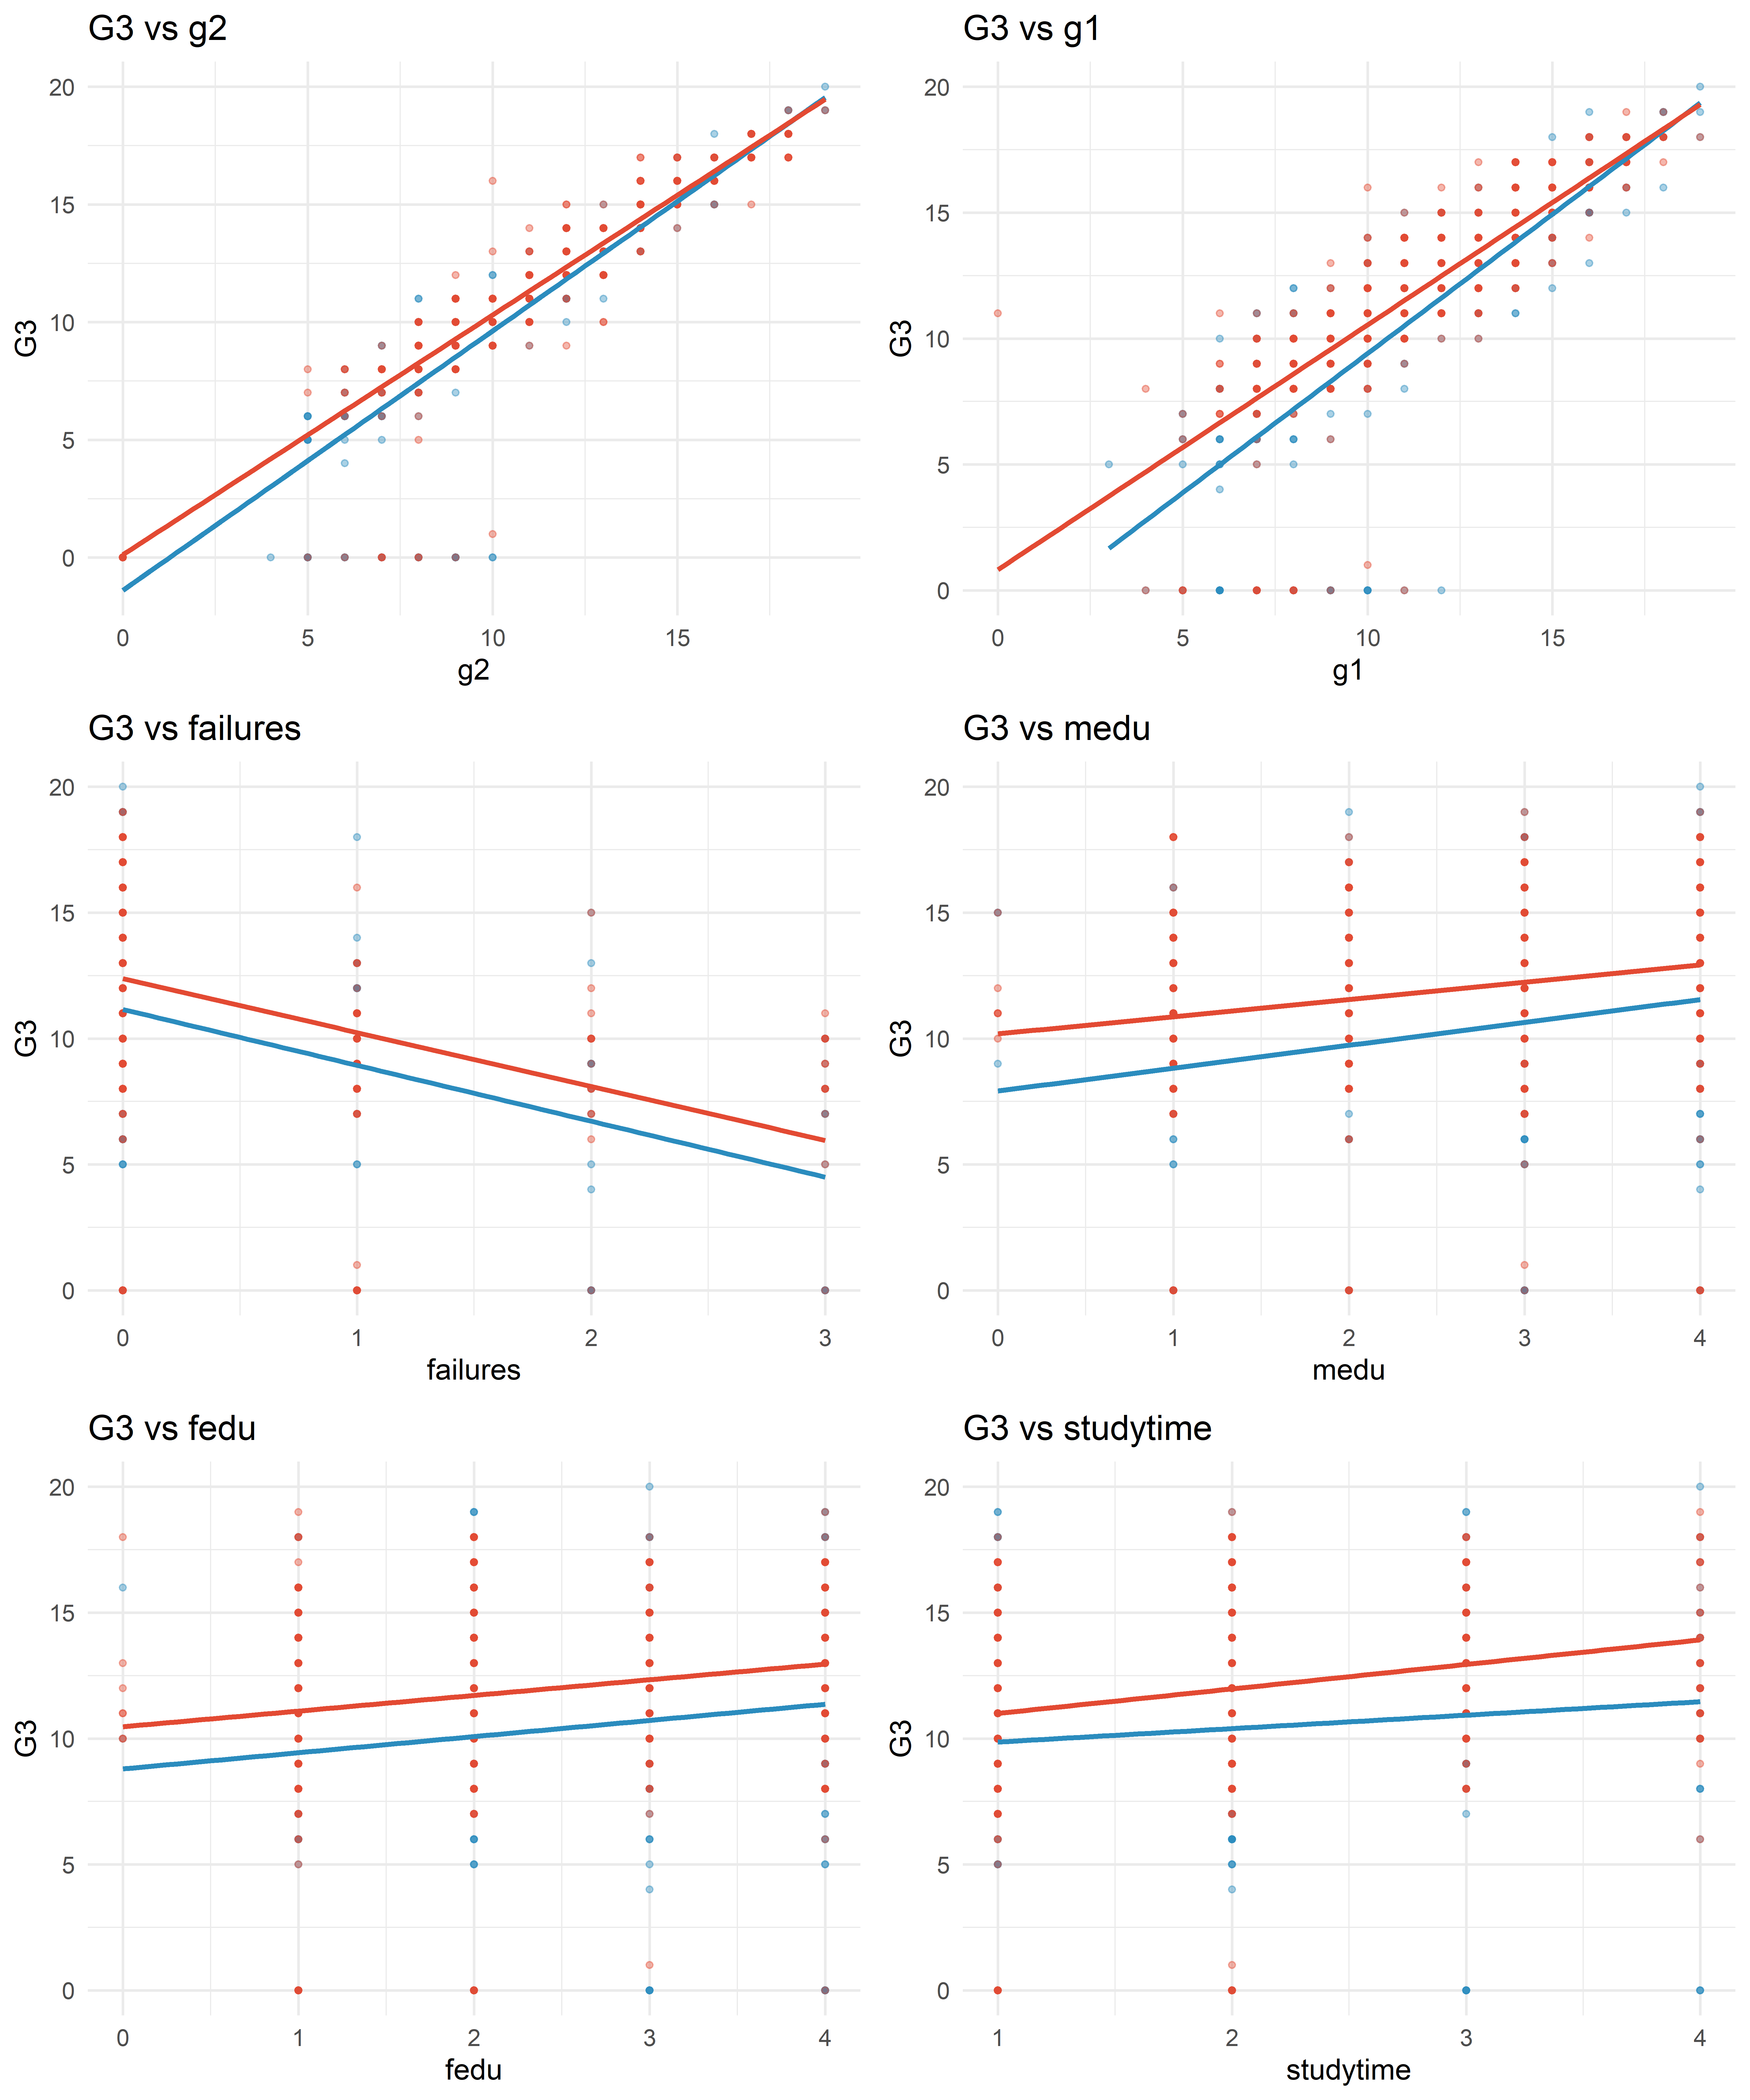
\includegraphics[keepaspectratio]{bookdown-demo_files/figure-latex/scatter-plots-1.pdf}}
\caption{\label{fig:scatter-plots}Relaciones de dispersión entre predictores numéricos y G3}
\end{figure}

\textbf{Deducciones de las Relaciones Numéricas:}

\begin{enumerate}
\def\labelenumi{\arabic{enumi}.}
\item
  \textbf{G2 y G1} muestran las correlaciones más fuertes con G3 (0.905), confirmando la progresión académica consistente.
\item
  \textbf{Failures} presenta correlación negativa fuerte, siendo un indicador crítico de riesgo académico.
\item
  \textbf{Study Time} muestra correlaciones positivas moderadas, validando la importancia del tiempo de estudio.
\end{enumerate}

\subsection{6.2 Variables Categóricas vs Rendimiento}\label{variables-categuxf3ricas-vs-rendimiento}

\begin{Shaded}
\begin{Highlighting}[]
\CommentTok{\# Variables categóricas clave}
\NormalTok{cats\_key }\OtherTok{\textless{}{-}} \FunctionTok{intersect}\NormalTok{(}\FunctionTok{c}\NormalTok{(}\StringTok{"sex"}\NormalTok{,}\StringTok{"address"}\NormalTok{,}\StringTok{"schoolsup"}\NormalTok{,}\StringTok{"higher"}\NormalTok{,}\StringTok{"internet"}\NormalTok{), }\FunctionTok{names}\NormalTok{(df\_all))}

\NormalTok{cat\_stats }\OtherTok{\textless{}{-}}\NormalTok{ purrr}\SpecialCharTok{::}\FunctionTok{map\_dfr}\NormalTok{(cats\_key, }\ControlFlowTok{function}\NormalTok{(var)\{}
\NormalTok{  df\_all }\SpecialCharTok{\%\textgreater{}\%}
    \FunctionTok{group\_by}\NormalTok{(subject, }\SpecialCharTok{!!}\FunctionTok{sym}\NormalTok{(var)) }\SpecialCharTok{\%\textgreater{}\%}
    \FunctionTok{summarise}\NormalTok{(}
      \AttributeTok{n =} \FunctionTok{n}\NormalTok{(),}
      \AttributeTok{mean\_g3 =} \FunctionTok{mean}\NormalTok{(g3),}
      \AttributeTok{sd\_g3 =} \FunctionTok{sd}\NormalTok{(g3),}
      \AttributeTok{.groups =} \StringTok{"drop"}
\NormalTok{    ) }\SpecialCharTok{\%\textgreater{}\%}
    \FunctionTok{mutate}\NormalTok{(}
      \AttributeTok{variable =}\NormalTok{ var,}
      \AttributeTok{category =} \FunctionTok{as.character}\NormalTok{(}\SpecialCharTok{!!}\FunctionTok{sym}\NormalTok{(var))}
\NormalTok{    ) }\SpecialCharTok{\%\textgreater{}\%}
    \CommentTok{\# nos quedamos solo con las 6 columnas que queremos}
    \FunctionTok{select}\NormalTok{(subject, variable, category, n, mean\_g3, sd\_g3)}
\NormalTok{\})}

\NormalTok{knitr}\SpecialCharTok{::}\FunctionTok{kable}\NormalTok{(}
  \FunctionTok{head}\NormalTok{(cat\_stats, }\DecValTok{10}\NormalTok{),}
  \AttributeTok{caption =} \StringTok{"Estadísticas de G3 por categorías (primeras 10 filas)"}\NormalTok{,}
  \AttributeTok{digits =} \DecValTok{2}\NormalTok{,}
  \AttributeTok{col.names =} \FunctionTok{c}\NormalTok{(}\StringTok{"Materia"}\NormalTok{, }\StringTok{"Variable"}\NormalTok{, }\StringTok{"Categoría"}\NormalTok{, }\StringTok{"N"}\NormalTok{, }\StringTok{"Media G3"}\NormalTok{, }\StringTok{"SD G3"}\NormalTok{)}
\NormalTok{)}
\end{Highlighting}
\end{Shaded}

\begin{table}

\caption{\label{tab:categorical-analysis}Estadísticas de G3 por categorías (primeras 10 filas)}
\centering
\begin{tabular}[t]{l|l|l|r|r|r}
\hline
Materia & Variable & Categoría & N & Media G3 & SD G3\\
\hline
Math & sex & F & 208 & 9.97 & 4.62\\
\hline
Math & sex & M & 187 & 10.91 & 4.50\\
\hline
Portuguese & sex & F & 383 & 12.25 & 3.12\\
\hline
Portuguese & sex & M & 266 & 11.41 & 3.32\\
\hline
Math & address & R & 88 & 9.51 & 4.56\\
\hline
Math & address & U & 307 & 10.67 & 4.56\\
\hline
Portuguese & address & R & 197 & 11.09 & 3.61\\
\hline
Portuguese & address & U & 452 & 12.26 & 2.99\\
\hline
Math & schoolsup & no & 344 & 10.56 & 4.77\\
\hline
Math & schoolsup & yes & 51 & 9.43 & 2.87\\
\hline
\end{tabular}
\end{table}

\begin{Shaded}
\begin{Highlighting}[]
\CommentTok{\# Boxplots para variables categóricas clave}
\NormalTok{plots\_cat }\OtherTok{\textless{}{-}} \FunctionTok{map}\NormalTok{(cats\_key, }\SpecialCharTok{\textasciitilde{}}\NormalTok{\{}
  \FunctionTok{ggplot}\NormalTok{(df\_all, }\FunctionTok{aes}\NormalTok{(.data[[.x]], g3, }\AttributeTok{fill =}\NormalTok{ subject)) }\SpecialCharTok{+}
    \FunctionTok{geom\_boxplot}\NormalTok{(}\AttributeTok{outlier.alpha =}\NormalTok{ .}\DecValTok{2}\NormalTok{, }\AttributeTok{width =}\NormalTok{ .}\DecValTok{6}\NormalTok{, }\AttributeTok{position =} \FunctionTok{position\_dodge}\NormalTok{(}\AttributeTok{width =}\NormalTok{ .}\DecValTok{75}\NormalTok{)) }\SpecialCharTok{+}
    \FunctionTok{geom\_point}\NormalTok{(}\FunctionTok{aes}\NormalTok{(}\AttributeTok{color =}\NormalTok{ subject),}
               \AttributeTok{position =} \FunctionTok{position\_jitterdodge}\NormalTok{(}\AttributeTok{jitter.width =}\NormalTok{ .}\DecValTok{15}\NormalTok{, }\AttributeTok{dodge.width =}\NormalTok{ .}\DecValTok{75}\NormalTok{),}
               \AttributeTok{size =}\NormalTok{ .}\DecValTok{6}\NormalTok{, }\AttributeTok{alpha =}\NormalTok{ .}\DecValTok{25}\NormalTok{, }\AttributeTok{show.legend =} \ConstantTok{FALSE}\NormalTok{) }\SpecialCharTok{+}
    \FunctionTok{scale\_fill\_manual}\NormalTok{(}\AttributeTok{values =}\NormalTok{ pal) }\SpecialCharTok{+} 
    \FunctionTok{scale\_color\_manual}\NormalTok{(}\AttributeTok{values =}\NormalTok{ pal) }\SpecialCharTok{+}
    \FunctionTok{labs}\NormalTok{(}\AttributeTok{title =} \FunctionTok{paste}\NormalTok{(}\StringTok{"G3 por"}\NormalTok{, .x), }\AttributeTok{x =}\NormalTok{ .x, }\AttributeTok{y =} \StringTok{"G3"}\NormalTok{) }\SpecialCharTok{+}
    \FunctionTok{theme}\NormalTok{(}\AttributeTok{legend.position =} \StringTok{"bottom"}\NormalTok{)}
\NormalTok{\})}

\FunctionTok{do.call}\NormalTok{(gridExtra}\SpecialCharTok{::}\NormalTok{grid.arrange, }\FunctionTok{c}\NormalTok{(plots\_cat, }\AttributeTok{ncol =} \DecValTok{2}\NormalTok{))}
\end{Highlighting}
\end{Shaded}

\begin{figure}
\centering
\pandocbounded{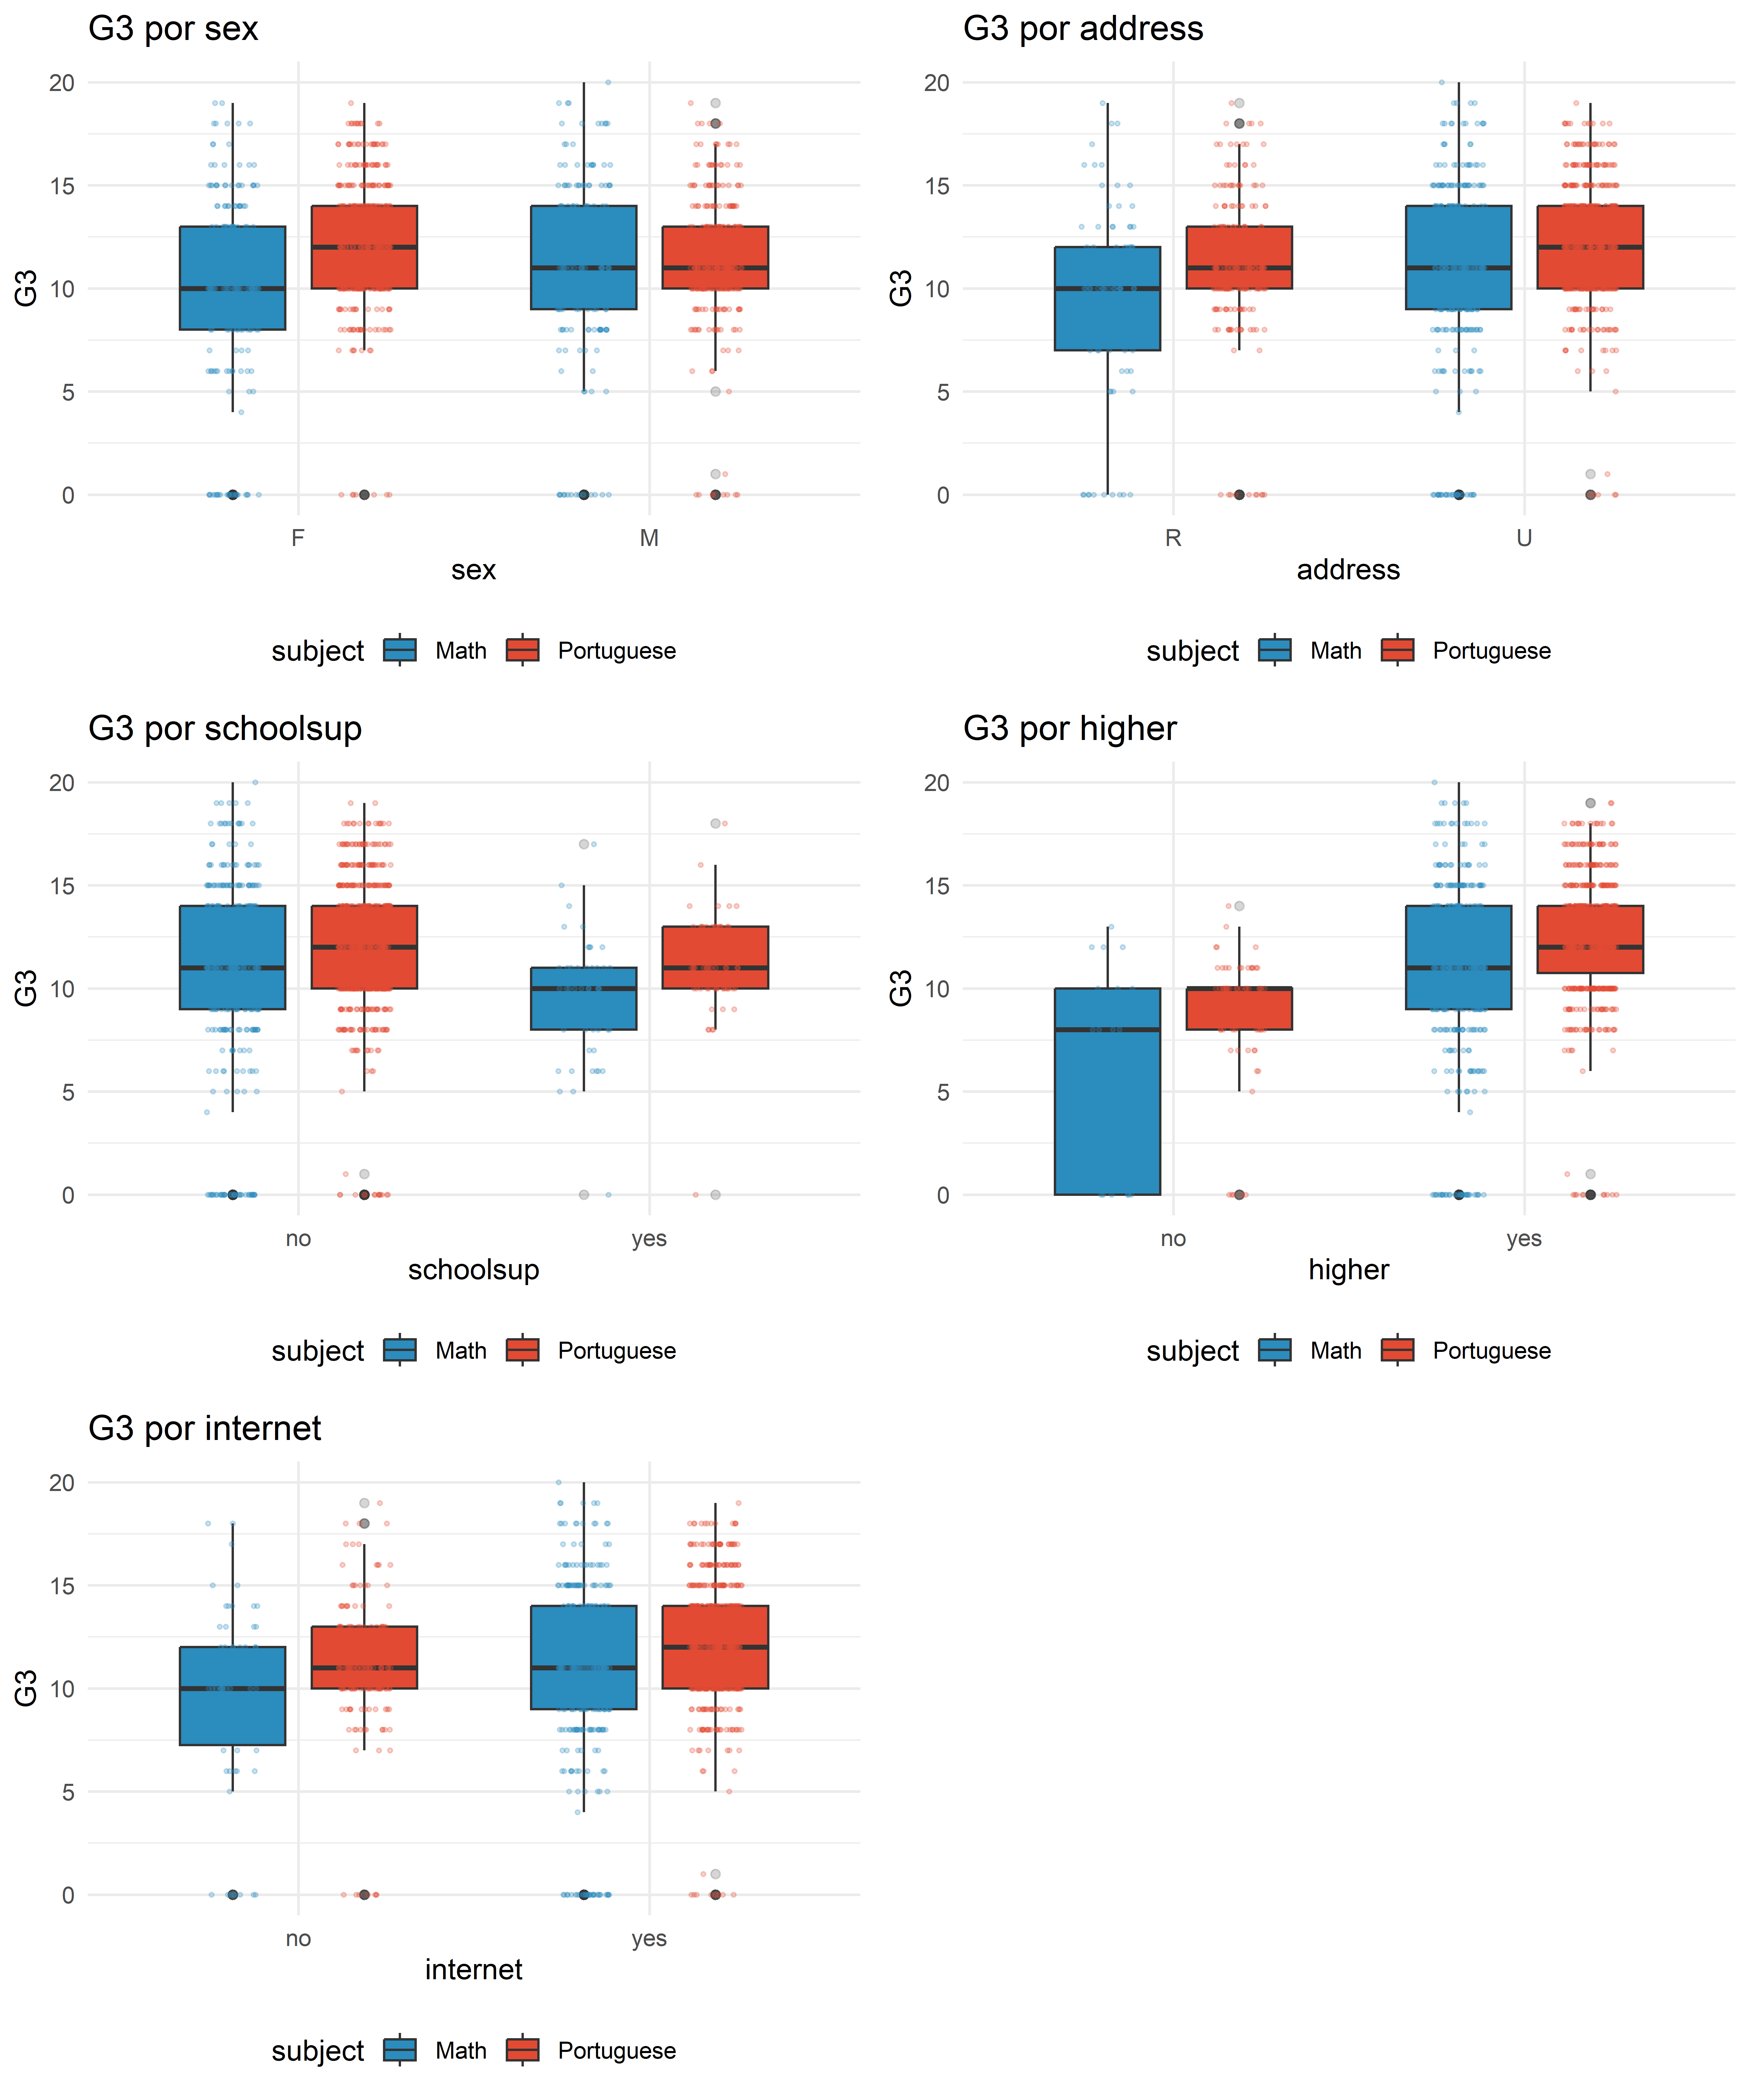
\includegraphics[keepaspectratio]{bookdown-demo_files/figure-latex/categorical-boxplots-1.pdf}}
\caption{\label{fig:categorical-boxplots}Distribución de G3 por variables categóricas clave}
\end{figure}

\textbf{Insights de Variables Categóricas:}

\begin{enumerate}
\def\labelenumi{\arabic{enumi}.}
\item
  \textbf{Higher Education Aspiration:} Los estudiantes que aspiran a educación superior muestran rendimiento significativamente mayor.
\item
  \textbf{Internet Access:} El acceso a internet se asocia con mejores calificaciones, sugiriendo ventajas en recursos educativos.
\item
  \textbf{School Support:} El apoyo escolar adicional muestra patrones complejos que requieren análisis más profundo.
\end{enumerate}

\begin{center}\rule{0.5\linewidth}{0.5pt}\end{center}

\section{7. Análisis de Éxito/Fracaso Académico}\label{anuxe1lisis-de-uxe9xitofracaso-acaduxe9mico}

\subsection{7.1 Definición de Éxito Académico}\label{definiciuxf3n-de-uxe9xito-acaduxe9mico}

\begin{Shaded}
\begin{Highlighting}[]
\CommentTok{\# Creación de variable binaria (aprobado/reprobado)}
\NormalTok{df\_bin }\OtherTok{\textless{}{-}}\NormalTok{ df\_all }\SpecialCharTok{\%\textgreater{}\%}
  \FunctionTok{mutate}\NormalTok{(}
    \AttributeTok{status =} \FunctionTok{factor}\NormalTok{(}
      \FunctionTok{if\_else}\NormalTok{(g3 }\SpecialCharTok{\textgreater{}=} \DecValTok{10}\NormalTok{, }\StringTok{"Aprobado"}\NormalTok{, }\StringTok{"Reprobado"}\NormalTok{),}
      \AttributeTok{levels =} \FunctionTok{c}\NormalTok{(}\StringTok{"Reprobado"}\NormalTok{, }\StringTok{"Aprobado"}\NormalTok{)}
\NormalTok{    )}
\NormalTok{  )}

\CommentTok{\# Estadísticas de aprobación}
\NormalTok{pass\_stats }\OtherTok{\textless{}{-}}\NormalTok{ df\_bin }\SpecialCharTok{\%\textgreater{}\%}
  \FunctionTok{group\_by}\NormalTok{(subject) }\SpecialCharTok{\%\textgreater{}\%}
  \FunctionTok{summarise}\NormalTok{(}
    \AttributeTok{total =} \FunctionTok{n}\NormalTok{(),}
    \AttributeTok{aprobados =} \FunctionTok{sum}\NormalTok{(status }\SpecialCharTok{==} \StringTok{"Aprobado"}\NormalTok{),}
    \AttributeTok{tasa\_aprobacion =} \FunctionTok{mean}\NormalTok{(status }\SpecialCharTok{==} \StringTok{"Aprobado"}\NormalTok{) }\SpecialCharTok{*} \DecValTok{100}\NormalTok{,}
    \AttributeTok{.groups =} \StringTok{"drop"}
\NormalTok{  )}

\FunctionTok{kable}\NormalTok{(pass\_stats,}
      \AttributeTok{caption =} \StringTok{"Tasas de aprobación por materia"}\NormalTok{,}
      \AttributeTok{digits =} \DecValTok{1}\NormalTok{,}
      \AttributeTok{col.names =} \FunctionTok{c}\NormalTok{(}\StringTok{"Materia"}\NormalTok{, }\StringTok{"Total"}\NormalTok{, }\StringTok{"Aprobados"}\NormalTok{, }\StringTok{"Tasa Aprobación (\%)"}\NormalTok{))}
\end{Highlighting}
\end{Shaded}

\begin{table}

\caption{\label{tab:binary-analysis}Tasas de aprobación por materia}
\centering
\begin{tabular}[t]{l|r|r|r}
\hline
Materia & Total & Aprobados & Tasa Aprobación (\%)\\
\hline
Math & 395 & 265 & 67.1\\
\hline
Portuguese & 649 & 549 & 84.6\\
\hline
\end{tabular}
\end{table}

\subsection{7.2 Factores Asociados al Éxito}\label{factores-asociados-al-uxe9xito}

\begin{Shaded}
\begin{Highlighting}[]
\CommentTok{\# Análisis de proporciones de éxito por categorías}
\NormalTok{success\_plots }\OtherTok{\textless{}{-}} \FunctionTok{map}\NormalTok{(cats\_key, }\SpecialCharTok{\textasciitilde{}}\NormalTok{\{}
  \FunctionTok{ggplot}\NormalTok{(df\_bin, }\FunctionTok{aes}\NormalTok{(.data[[.x]], }\AttributeTok{fill =}\NormalTok{ status)) }\SpecialCharTok{+}
    \FunctionTok{geom\_bar}\NormalTok{(}\AttributeTok{position =} \StringTok{"fill"}\NormalTok{) }\SpecialCharTok{+}
    \FunctionTok{facet\_wrap}\NormalTok{(}\SpecialCharTok{\textasciitilde{}}\NormalTok{subject) }\SpecialCharTok{+}
    \FunctionTok{scale\_fill\_manual}\NormalTok{(}\AttributeTok{values =} \FunctionTok{c}\NormalTok{(}\StringTok{"Reprobado"} \OtherTok{=} \StringTok{"\#D9D9D9"}\NormalTok{, }\StringTok{"Aprobado"} \OtherTok{=} \StringTok{"\#31A354"}\NormalTok{)) }\SpecialCharTok{+}
    \FunctionTok{scale\_y\_continuous}\NormalTok{(}\AttributeTok{labels =}\NormalTok{ percent) }\SpecialCharTok{+}
    \FunctionTok{labs}\NormalTok{(}\AttributeTok{title =} \FunctionTok{paste}\NormalTok{(}\StringTok{"Proporción de aprobados por"}\NormalTok{, .x), }
         \AttributeTok{x =}\NormalTok{ .x, }\AttributeTok{y =} \StringTok{"Proporción"}\NormalTok{) }\SpecialCharTok{+}
    \FunctionTok{theme}\NormalTok{(}\AttributeTok{legend.position =} \StringTok{"bottom"}\NormalTok{)}
\NormalTok{\})}

\FunctionTok{do.call}\NormalTok{(gridExtra}\SpecialCharTok{::}\NormalTok{grid.arrange, }\FunctionTok{c}\NormalTok{(success\_plots[}\DecValTok{1}\SpecialCharTok{:}\DecValTok{4}\NormalTok{], }\AttributeTok{ncol =} \DecValTok{2}\NormalTok{))}
\end{Highlighting}
\end{Shaded}

\begin{figure}
\centering
\pandocbounded{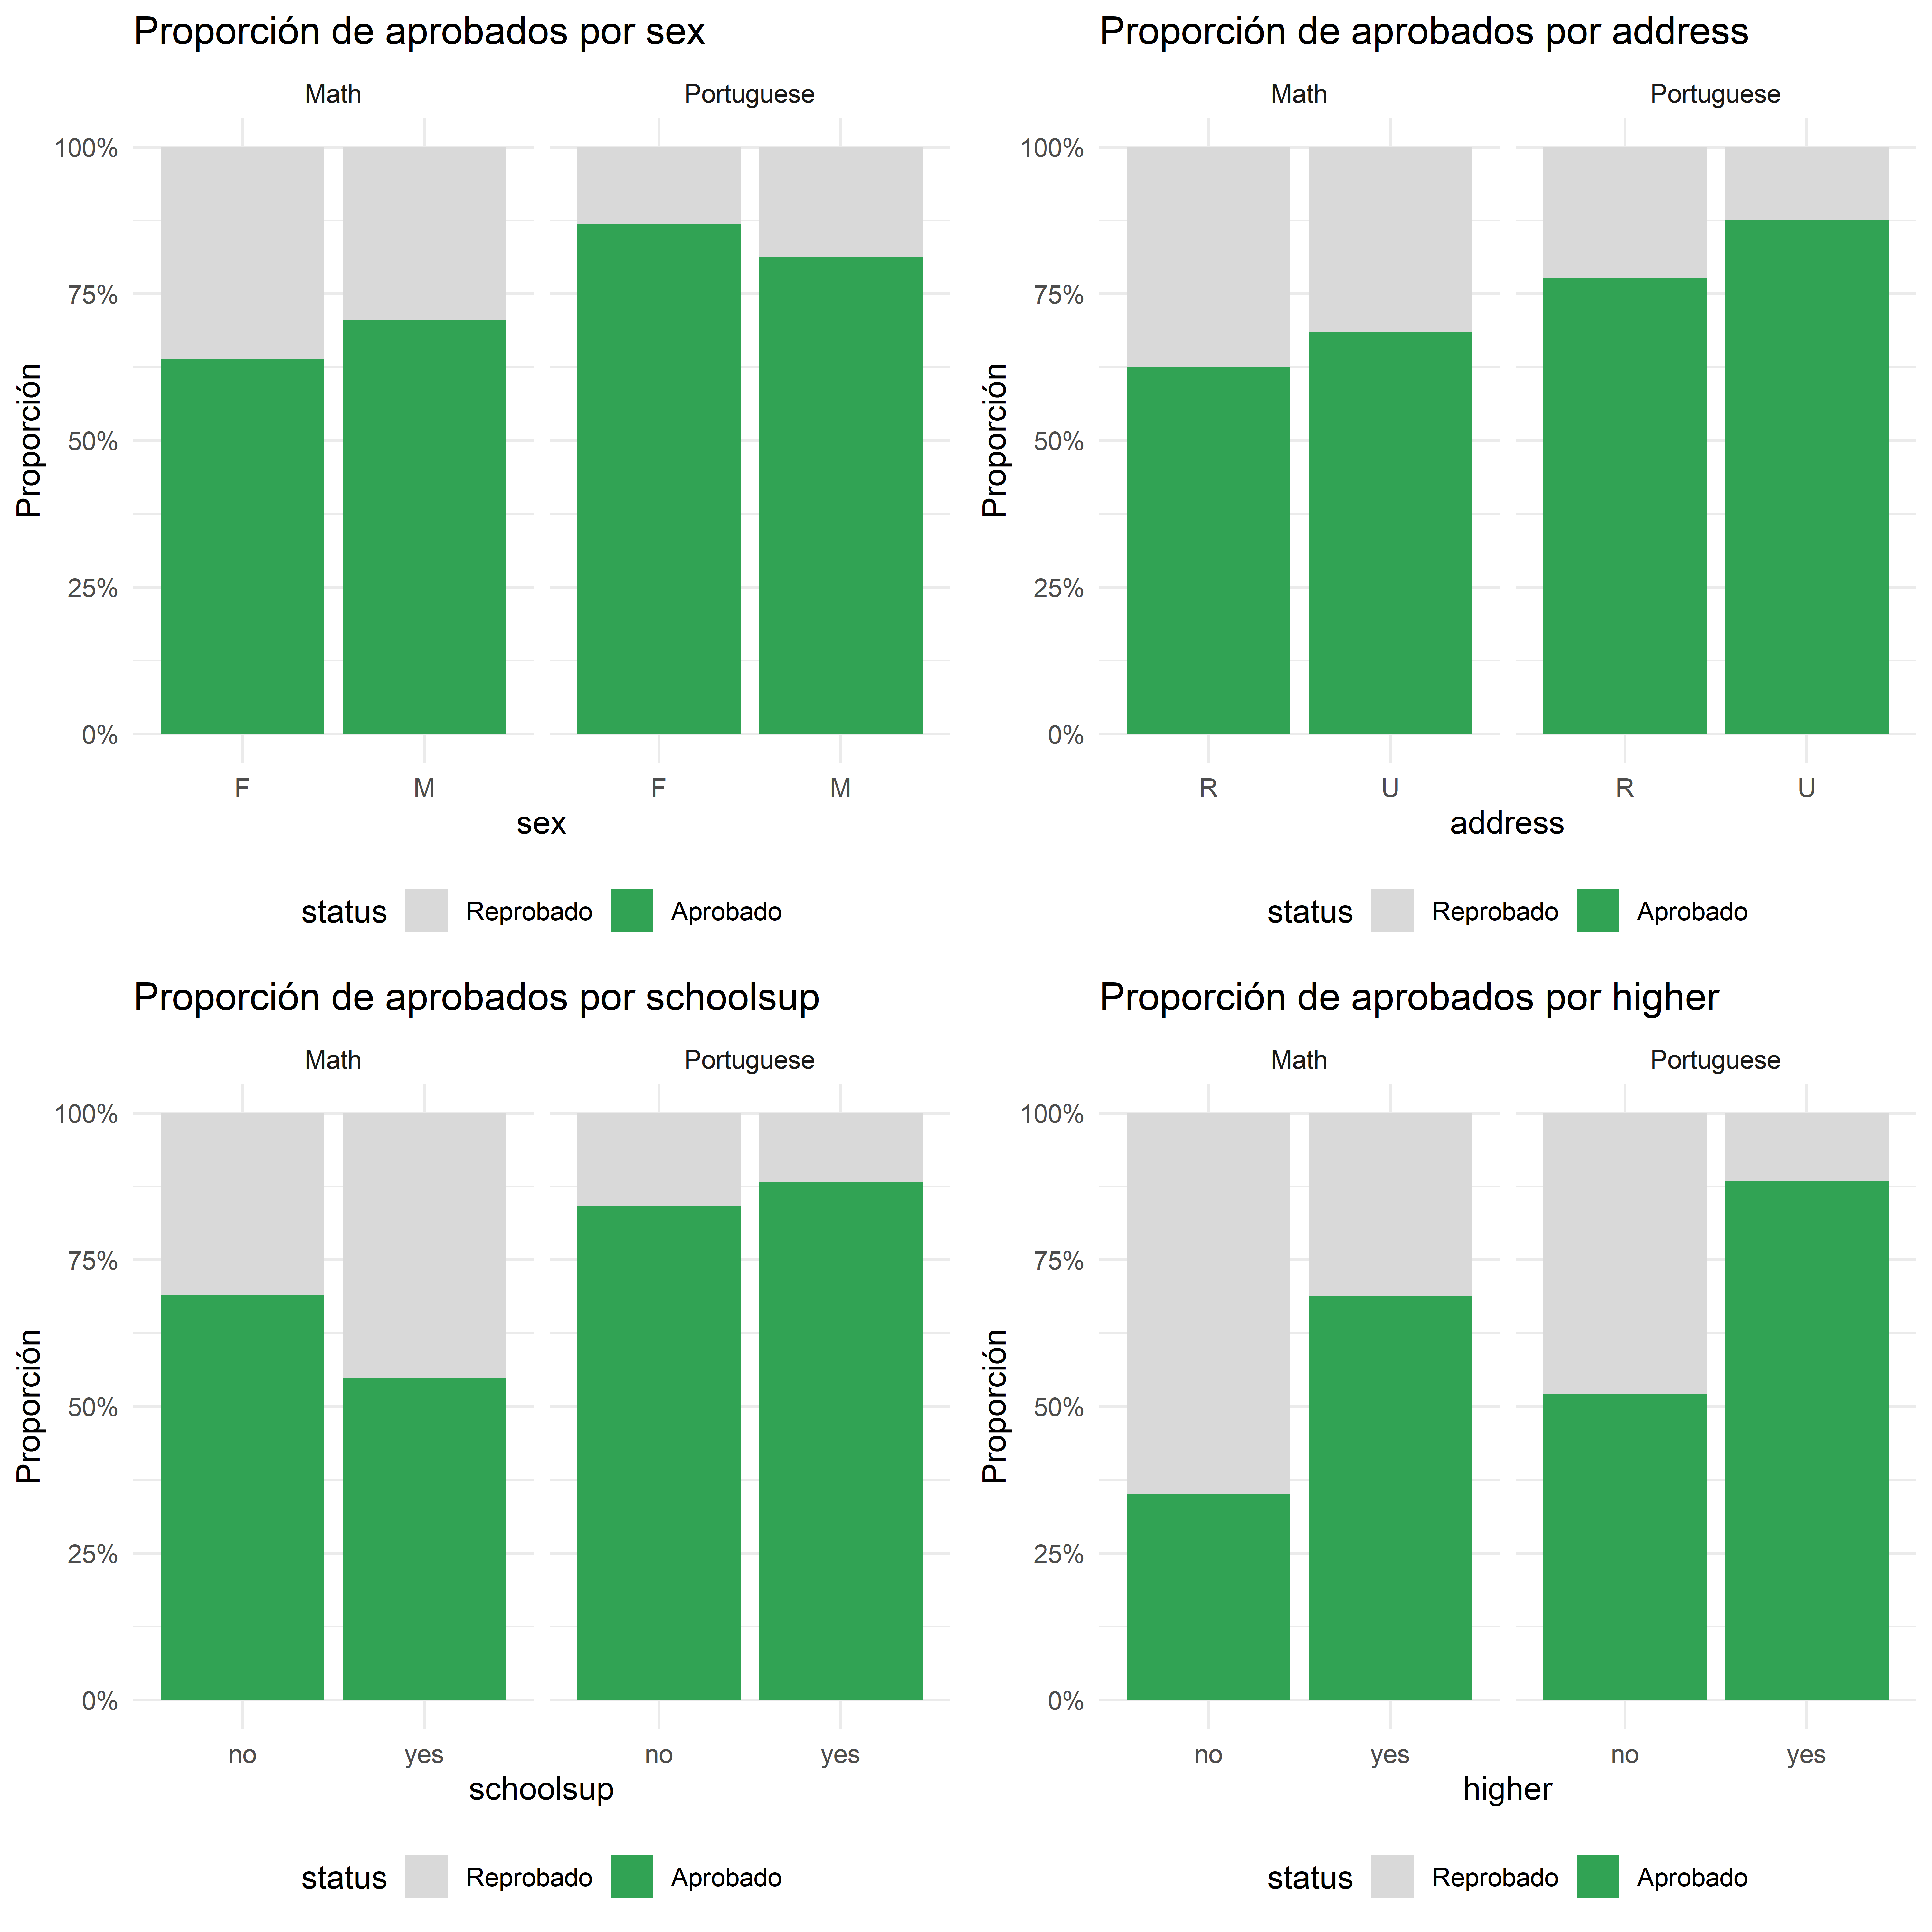
\includegraphics[keepaspectratio]{bookdown-demo_files/figure-latex/success-factors-1.pdf}}
\caption{\label{fig:success-factors}Factores asociados al éxito académico}
\end{figure}

\begin{Shaded}
\begin{Highlighting}[]
\CommentTok{\# Análisis de variables numéricas por estado}
\NormalTok{nums\_success }\OtherTok{\textless{}{-}} \FunctionTok{setdiff}\NormalTok{(nums\_key, }\StringTok{"g3"}\NormalTok{)[}\DecValTok{1}\SpecialCharTok{:}\DecValTok{4}\NormalTok{]  }\CommentTok{\# Top 4 variables}

\NormalTok{numeric\_success\_plots }\OtherTok{\textless{}{-}} \FunctionTok{map}\NormalTok{(nums\_success, }\SpecialCharTok{\textasciitilde{}}\NormalTok{\{}
  \FunctionTok{ggplot}\NormalTok{(df\_bin, }\FunctionTok{aes}\NormalTok{(status, .data[[.x]], }\AttributeTok{fill =}\NormalTok{ status)) }\SpecialCharTok{+}
    \FunctionTok{geom\_boxplot}\NormalTok{(}\AttributeTok{outlier.alpha =}\NormalTok{ .}\DecValTok{25}\NormalTok{, }\AttributeTok{width =}\NormalTok{ .}\DecValTok{5}\NormalTok{) }\SpecialCharTok{+}
    \FunctionTok{facet\_wrap}\NormalTok{(}\SpecialCharTok{\textasciitilde{}}\NormalTok{subject, }\AttributeTok{scales =} \StringTok{"free\_y"}\NormalTok{) }\SpecialCharTok{+}
    \FunctionTok{scale\_fill\_manual}\NormalTok{(}\AttributeTok{values =} \FunctionTok{c}\NormalTok{(}\StringTok{"Reprobado"} \OtherTok{=} \StringTok{"\#FDD0A2"}\NormalTok{, }\StringTok{"Aprobado"} \OtherTok{=} \StringTok{"\#9ECAE1"}\NormalTok{)) }\SpecialCharTok{+}
    \FunctionTok{guides}\NormalTok{(}\AttributeTok{fill =} \StringTok{"none"}\NormalTok{) }\SpecialCharTok{+}
    \FunctionTok{labs}\NormalTok{(}\AttributeTok{title =} \FunctionTok{paste}\NormalTok{(.x, }\StringTok{"por estado académico"}\NormalTok{), }\AttributeTok{x =} \ConstantTok{NULL}\NormalTok{, }\AttributeTok{y =}\NormalTok{ .x)}
\NormalTok{\})}

\FunctionTok{do.call}\NormalTok{(gridExtra}\SpecialCharTok{::}\NormalTok{grid.arrange, }\FunctionTok{c}\NormalTok{(numeric\_success\_plots, }\AttributeTok{ncol =} \DecValTok{2}\NormalTok{))}
\end{Highlighting}
\end{Shaded}

\begin{figure}
\centering
\pandocbounded{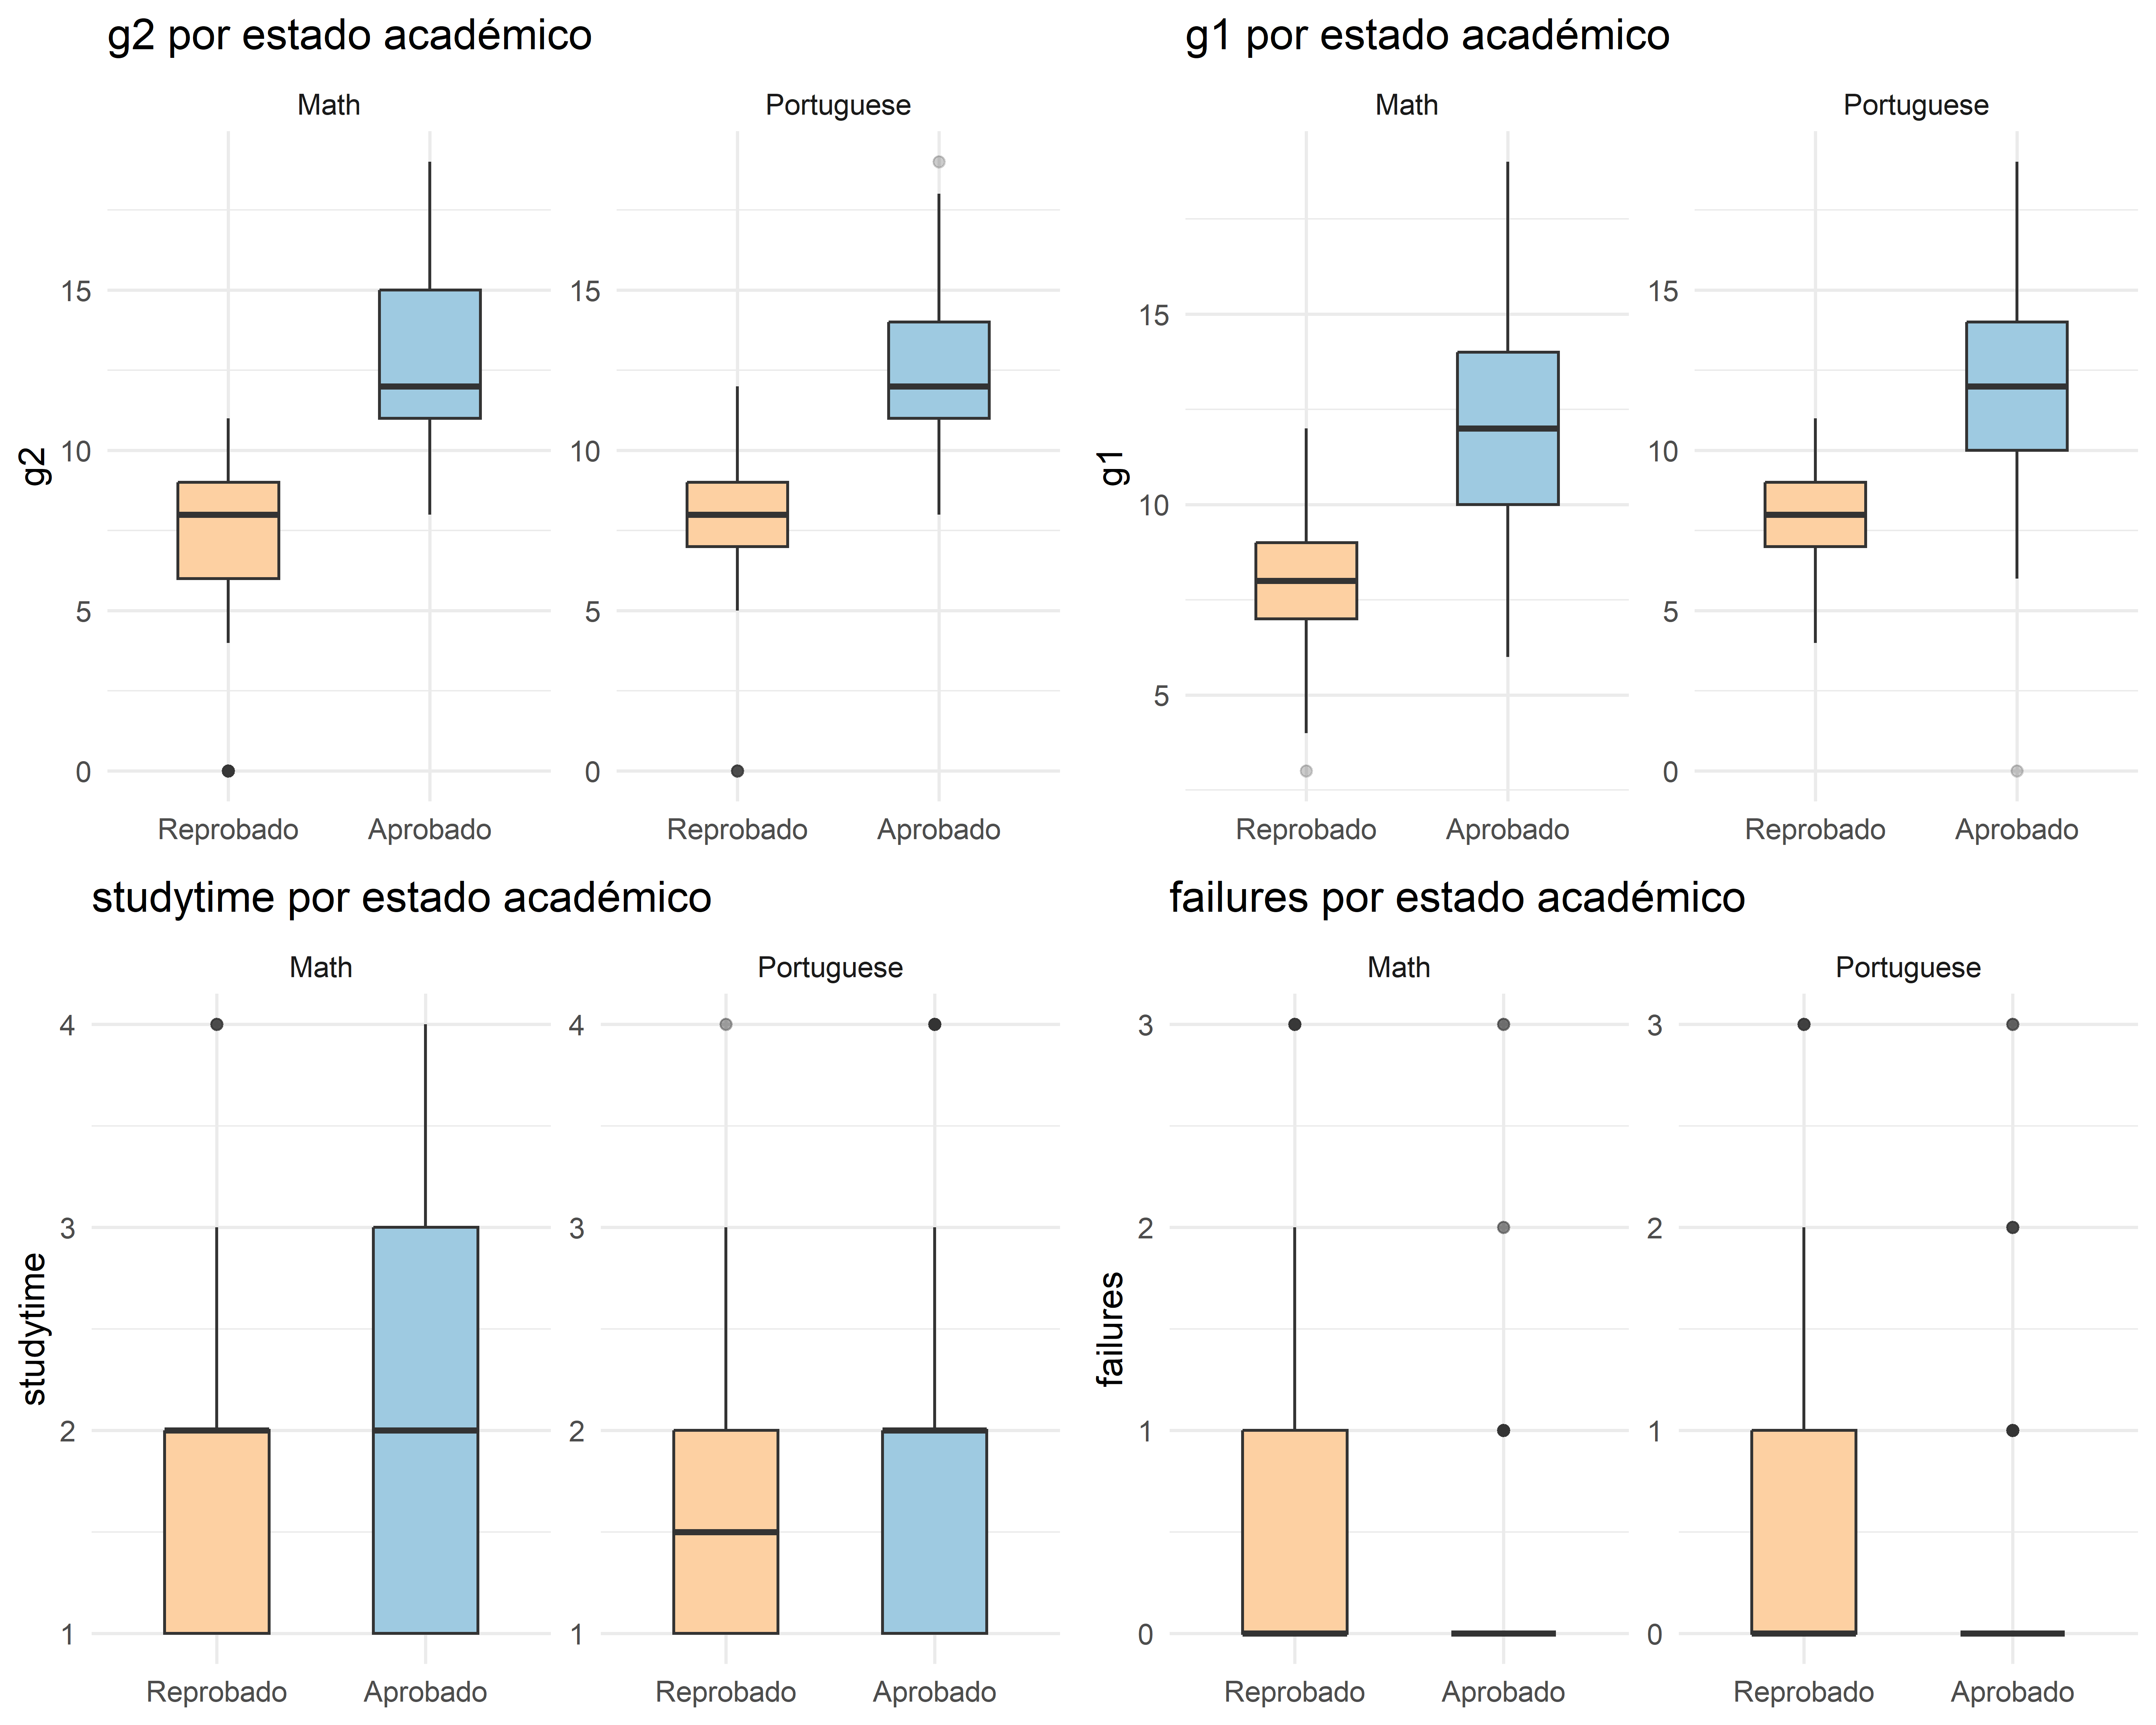
\includegraphics[keepaspectratio]{bookdown-demo_files/figure-latex/numeric-success-1.pdf}}
\caption{\label{fig:numeric-success}Distribución de variables numéricas por estado académico}
\end{figure}

\textbf{Factores Críticos de Éxito Identificados:}

\begin{enumerate}
\def\labelenumi{\arabic{enumi}.}
\item
  \textbf{Aspiraciones Educativas:} Los estudiantes que planean continuar con educación superior tienen tasas de aprobación 80.7\% vs 48.3\% de quienes no planean hacerlo.
\item
  \textbf{Historial Académico:} Los estudiantes sin reprobaciones previas muestran tasas de éxito significativamente superiores.
\item
  \textbf{Acceso a Recursos:} El acceso a internet y apoyo educativo se correlaciona positivamente con el éxito académico.
\end{enumerate}

\begin{center}\rule{0.5\linewidth}{0.5pt}\end{center}

\section{8. Conclusiones y Recomendaciones}\label{conclusiones-y-recomendaciones}

\subsection{8.1 Hallazgos Principales}\label{hallazgos-principales}

\subsubsection{8.1.1 Diferencias por Materia}\label{diferencias-por-materia}

\begin{itemize}
\tightlist
\item
  \textbf{Portugués presenta mejor rendimiento general} que Matemáticas (media: 11.91 vs 10.42)
\item
  \textbf{Matemáticas muestra mayor variabilidad} en las calificaciones, sugiriendo polarización en el rendimiento
\item
  Las \textbf{correlaciones entre predictores y G3 son consistentes} entre materias, indicando factores comunes de éxito
\end{itemize}

\subsubsection{8.1.2 Predictores Clave del Rendimiento}\label{predictores-clave-del-rendimiento}

\begin{enumerate}
\def\labelenumi{\arabic{enumi}.}
\tightlist
\item
  \textbf{Rendimiento previo (G1, G2):} Factor más fuerte (r \textgreater{} 0.8)
\item
  \textbf{Historial de reprobaciones:} Predictor negativo crítico
\item
  \textbf{Aspiraciones educativas:} Diferenciador importante del éxito
\item
  \textbf{Acceso a recursos tecnológicos:} Ventaja competitiva
\item
  \textbf{Tiempo de estudio:} Correlación positiva moderada pero consistente
\end{enumerate}

\subsubsection{8.1.3 Patrones de Riesgo Académico}\label{patrones-de-riesgo-acaduxe9mico}

\begin{itemize}
\tightlist
\item
  Estudiantes con \textbf{múltiples reprobaciones} tienen probabilidades extremadamente bajas de éxito
\item
  La \textbf{combinación de bajo apoyo familiar y escolar} crea vulnerabilidad académica
\item
  \textbf{Altas ausencias} se asocian sistemáticamente con bajo rendimiento
\end{itemize}

\begin{center}\rule{0.5\linewidth}{0.5pt}\end{center}

\section{9. Referencias y Metodología}\label{referencias-y-metodologuxeda}

\textbf{Dataset:} P. Cortez and A. Silva. Using Data Mining to Predict Secondary School Student Performance. In A. Brito and J. Teixeira Eds., Proceedings of 5th FUture BUsiness TEChnology Conference (FUBUTEC 2008) pp.~5-12, Porto, Portugal, April, 2008, EUROSIS, ISBN 978-9077381-39-7.

\textbf{Herramientas utilizadas:}
- R R version 4.5.1 (2025-06-13 ucrt)
- Tidyverse 2.0.0
- GGally 2.3.0

\begin{center}\rule{0.5\linewidth}{0.5pt}\end{center}

\end{document}
